%%%%%%%%%%%%%%%%%%%%%%%%%%%%%%%%%%%%%%%%%%%%%%%%%%%%%%%%%%%%%%%%%%
%%%%%%%%%%%%%%%%%%%%%%%%%%%%%%%%%%%%%%%%%%%%%%%%%%%%%%%%%%%%%%%%%%
%\pagestyle{myheadings} \markright{Daniel Wollschläger \hfill Grundlagen der Datenanalyse mit R}
\chapter{Regressionsmodelle für kategoriale Daten und Zähldaten}
\label{sec:glm}
%%%%%%%%%%%%%%%%%%%%%%%%%%%%%%%%%%%%%%%%%%%%%%%%%%%%%%%%%%%%%%%%%%
%%%%%%%%%%%%%%%%%%%%%%%%%%%%%%%%%%%%%%%%%%%%%%%%%%%%%%%%%%%%%%%%%%

\index{verallgemeinertes lineares Modell}
Das Modell der linearen Regression und Varianzanalyse (Abschn.\ \ref{sec:regrMult}, \ref{sec:CRp}, \ref{sec:multALMregr}) lässt sich zum verallgemeinerten linearen Modell (GLM, \emph{generalized linear model}) erweitern, das auch für Daten einer kategorialen vorherzusagenden Variable $Y$ geeignet ist.\footnote{Abschnitt \ref{sec:lmLongitudinal} gibt Hinweise auf gemischte Regressionsmodelle und verallgemeinerte Schätzgleichungen (GEE) für abhängige Daten -- etwa durch Messwiederholung oder Clusterung, die analog auf kategoriale Zielgrößen übertragen werden können.} Als Prädiktoren lassen sich sowohl kontinuierliche Variablen als auch Gruppierungsfaktoren einsetzen. Ein Spezialfall ist die logistische Regression für dichotome $Y$ (codiert als $0$ und $1$). Im Vergleich zur Vorhersage quantitativer Variablen in der linearen Regression wird an diesem Beispiel zunächst folgende Schwierigkeit deutlich (für Details vgl.\ \citeNP{Faraway2006,Fox2002}):

Eine lineare Funktion von $p$ Prädiktoren $X_{j}$ der Form $\beta_{0} + \beta_{1} X_{1} + \dots + \beta_{j} X_{j} + \dots + \beta_{p} X_{p}$ kann bei einem unbeschränkten Definitionsbereich beliebige Werte im Intervall $(-{\infty}, +{\infty})$ annehmen. Es können sich durch die Modellgleichung also Werte ergeben, die weder von $Y$ selbst, noch vom Erwartungswert $E(Y)$ angenommen werden können. Dabei ist $E(Y)$ für dichotome $Y$ die Wahrscheinlichkeit eines Treffers $P(Y = 1)$, die im Intervall $[0, 1]$ liegt.

Dagegen ist die lineare Modellierung von\index{Logit-Funktion} $\text{logit}(P) = \ln \frac{P}{1-P}$ möglich, dem natürlichen Logarithmus des Wettquotienten, der Werte im Intervall $(-{\infty}, +{\infty})$ annimmt. Man setzt nun $\ln \frac{P}{1-P} = \beta_{0} + \beta_{1} X_{1} + \dots + \beta_{p} X_{p}$ als gültiges Modell voraus und fasst die rechte Seite der Gleichung als \emph{linearen Prädiktor} $\bm{X} \bm{\beta}$ zusammen (Abschn.\ \ref{sec:multALMregr}). Dann ist $P$ mit der Verteilungsfunktion der standardisierten logistischen Verteilung als Umkehrfunktion der Logit-Funktion als $P = \frac{\euler^{\bm{X} \bm{\beta}}}{1+\euler^{\bm{X} \bm{\beta}}} = \frac{1}{1+\euler^{-\bm{X} \bm{\beta}}}$ identifizierbar. Solche Transformationen des eigentlich vorherzusagenden Parameters, die eine lineare Modellierung ermöglichen, heißen \emph{Link-Funktion} $g(\cdot)$. Sie müssen u.\,a.\ eine Umkehrfunktion $g^{-1}(\cdot)$ besitzen, so dass $g(E(Y)) = \bm{X} \bm{\beta}$ und $E(Y) = g^{-1}(\bm{X} \bm{\beta})$ gilt.

Verkürzt gesprochen wird im GLM anders als im allgemeinen linearen Modell nur $E(Y)$ über die Link-Funktion linear modelliert, nicht $Y$ selbst. Es ist deshalb notwendig, die angenommene Form der bedingten Verteilung von $Y$ für gegebene Prädiktorwerte explizit anzugeben (Abschn.\ \ref{sec:multALM}). Mit dieser Form liegt auch die Varianz der Verteilung in Abhängigkeit von $E(Y)$ fest. Die bedingte Verteilung muss aus der natürlichen Exponentialfamilie stammen und wird mit einer Link-Funktion kombiniert, die $E(Y)$ mit dem linearen Prädiktor $\bm{X} \bm{\beta}$ in Beziehung setzt. Sind mehrere Link-Funktionen mit einer bedingten Verteilungsform kombinierbar, ist eine davon die \emph{kanonische} Link-Funktion mit besonderen statistischen Eigenschaften.

Die lineare Regression ist ein Spezialfall des GLM, bei dem von bedingter Normalverteilung von $Y$ ausgegangen wird (Abschn.\ \ref{sec:multALMpred}, Abb.\ \ref{fig:regrHomSc}) und $E(Y)$ zudem nicht durch eine Link-Funktion transformiert werden muss, um linear modellierbar zu sein. Anders als in der linearen Regression werden die Parameter $\beta_{j}$ im GLM über die Maximum-Likelihood-Methode geschätzt (Abschn.\ \ref{sec:glmConvergence}). In den folgenden Abschnitten sollen die logistische, ordinale, multinomiale und Poisson-Regression ebenso vorgestellt werden wie log-lineare Modelle. Für die Visualisierung kategorialer Daten s.\ Abschn.\ \ref{sec:barplot} sowie das Paket \lstinline!vcd!\index[pack]{vcd@\lstinline{vcd}|textbf} \cite{Meyer2009b}.

%%%%%%%%%%%%%%%%%%%%%%%%%%%%%%%%%%%%%%%%%%%%%%%%%%%%%%%%%%%%%%%%%%
%%%%%%%%%%%%%%%%%%%%%%%%%%%%%%%%%%%%%%%%%%%%%%%%%%%%%%%%%%%%%%%%%%
\section{Logistische Regression}
\label{sec:regrLog}
%%%%%%%%%%%%%%%%%%%%%%%%%%%%%%%%%%%%%%%%%%%%%%%%%%%%%%%%%%%%%%%%%%
%%%%%%%%%%%%%%%%%%%%%%%%%%%%%%%%%%%%%%%%%%%%%%%%%%%%%%%%%%%%%%%%%%

\index{Regression!logistische}
\index{logistische Regression|see{Regression}}
In der logistischen Regression für dichotome Daten wird als bedingte Verteilung von $Y$ die Binomialverteilung angenommen, die kanonische Link-Funktion ist die Logit-Funktion. Die bedingten Verteilungen sind dann durch $E(Y) = P$ vollständig festgelegt, da ihre Varianz gleich $n_{i} \, P \, (1-P)$ ist. Dabei ist $n_{i}$ die Anzahl der dichotomen Messwerte für dieselbe Kombination von Prädiktorwerten.

%%%%%%%%%%%%%%%%%%%%%%%%%%%%%%%%%%%%%%%%%%%%%%%%%%%%%%%%%%%%%%%%%%
%%%%%%%%%%%%%%%%%%%%%%%%%%%%%%%%%%%%%%%%%%%%%%%%%%%%%%%%%%%%%%%%%%
\subsection{Modell für dichotome Daten anpassen}
\label{sec:glmFit}
%%%%%%%%%%%%%%%%%%%%%%%%%%%%%%%%%%%%%%%%%%%%%%%%%%%%%%%%%%%%%%%%%%
%%%%%%%%%%%%%%%%%%%%%%%%%%%%%%%%%%%%%%%%%%%%%%%%%%%%%%%%%%%%%%%%%%

Die Anpassung einer logistischen Regression geschieht mit der \lstinline!glm()!\index[func]{glm()@\lstinline{glm()}} Funktion, mit der allgemein GLM-Modelle spezifiziert werden können.\footnote{Für die\index{Regression!bedingte logistische} bedingte logistische Regression bei Stratifizierung der Beobachtungen vgl.\ \lstinline!clogit()!\index[func]{clogit()@\lstinline{clogit()}} aus dem Paket \index[pack]{survival@\lstinline{survival}|textbf} \lstinline!survival! \cite{Therneau2012a}.} Hier sei zunächst der Fall betrachtet, dass die erhobenen Daten als dichotome Variable vorliegen.
\begin{lstlisting}
glm(formula=<<Modellformel>>, family=<<Verteilung>>, data=<<Datensatz>>,
    subset=<<Indexvektor>>)
\end{lstlisting}

Unter \lstinline!formula! wird eine Modellformel \lstinline!<<Zielgröße>> ~ <<Prädiktoren>>! wie mit \lstinline!lm()! formuliert, wobei sowohl quantitative wie kategoriale Variablen als Prädiktoren möglich sind. Stammen die Variablen aus einem Datensatz, ist dieser unter \lstinline!data! zu nennen. Die Zielgröße muss ein Objekt der Klasse \lstinline!factor! mit zwei Stufen sein, die Auftretenswahrscheinlichkeit $P$ bezieht sich auf die zweite Faktorstufe. Weiter ist unter \lstinline!family! ein Objekt anzugeben, das die für die Zielgröße angenommene bedingte Verteilung sowie die Link-Funktion benennt (vgl.\ \lstinline!?family!). Im Fall der logistischen Regression ist dieses Argument auf \lstinline!binomial(link="logit")! zu setzen. Das Argument \lstinline!subset! erlaubt es, nur eine Teilmenge der Fälle einfließen zu lassen. Es erwartet einen numerischen oder logischen Indexvektor, der sich auf die Zeilen des Datensatzes bezieht.

Als Beispiel sei jenes aus der Kovarianzanalyse herangezogen (Abschn.\ \ref{sec:ancova}), wobei hier vorhergesagt werden soll, ob die Depressivität nach der Behandlung über dem Median liegt. Die Beziehung zwischen der Depressivität vor und nach der Behandlung in den drei Gruppen soll dabei zunächst über ein Diagramm mit dem nonparametrisch geschätzten Verlauf der Trefferwahrscheinlichkeit veranschaulicht werden, das \lstinline!cdplot(<<Modellformel>>)!\index[func]{cdplot()@\lstinline{cdplot()}} erzeugt (\emph{conditional density plot}, Abb.\ \ref{fig:regrLogCD}).
\begin{lstlisting}
# Median-Split: Umwandlung quantitative Zielgröße in dichotomen Faktor
> dfAncova <- transform(dfAncova,
+              postFac=cut(DVpost, breaks=c(-Inf, median(DVpost), Inf),
+                          labels=c("lo", "hi")))

# conditional density plot der Zielgröße in den drei Gruppen
> cdplot(postFac ~ DVpre, data=dfAncova, subset=(IV == "SSRI"),
+        main="Geschätzte Kategorien-Wkt. SSRI")

> cdplot(postFac ~ DVpre, data=dfAncova, subset=(IV == "Placebo"),
+        main="Geschätzte Kategorien-Wkt. Placebo")

> cdplot(postFac ~ DVpre, data=dfAncova, subset=(IV == "WL"),
+        main="Geschätzte Kategorien-Wkt. WL")
\end{lstlisting}

\begin{figure}[ht]
\centering
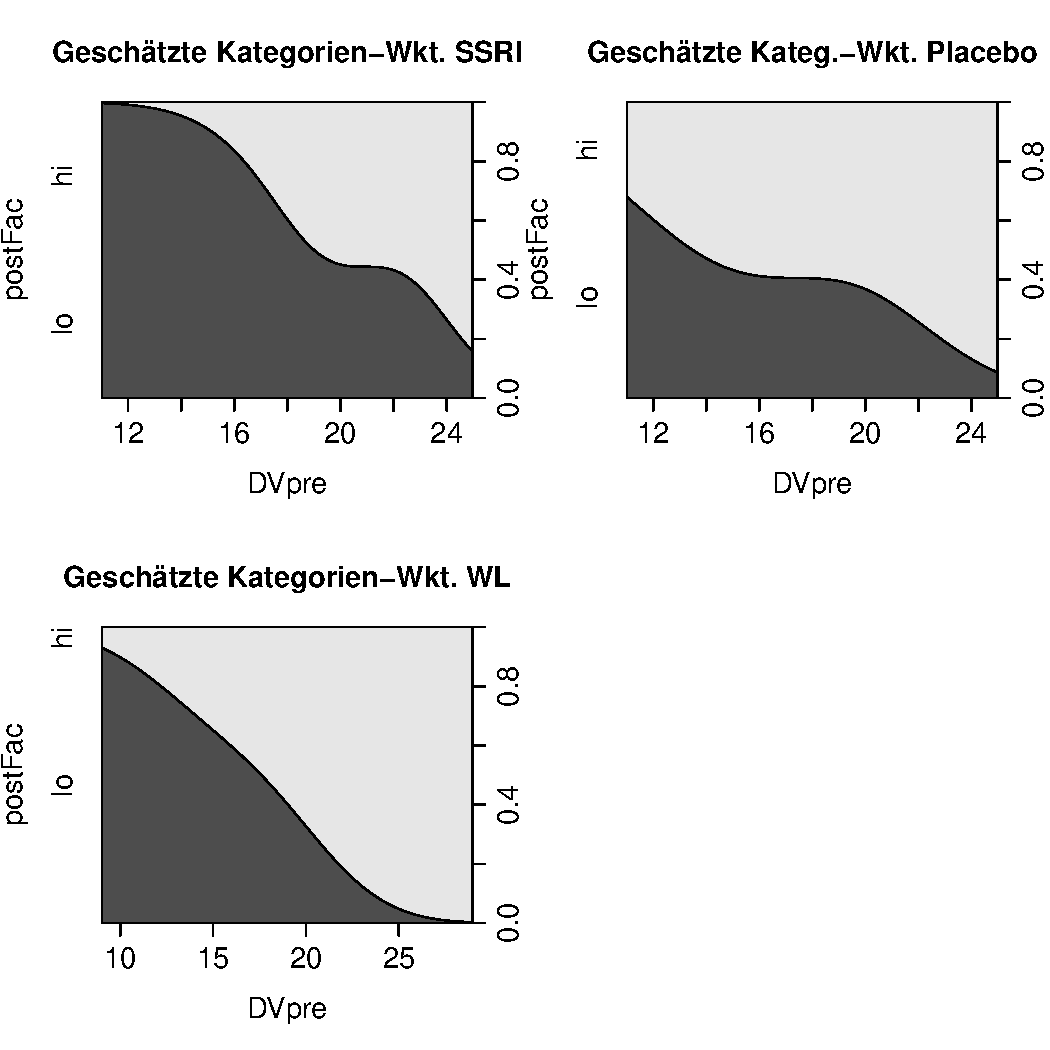
\includegraphics[width=12.5cm]{regrLogCD}
\vspace*{-1em}
\caption{Nonparametrisch geschätzte Kategorienwahrscheinlichkeiten in Abhängigkeit vom Prädiktor in drei Behandlungsgruppen}
\label{fig:regrLogCD}
\end{figure}

\begin{lstlisting}
# Anpassung des logistischen Regressionsmodells
> (glmFit <- glm(postFac ~ DVpre + IV, family=binomial(link="logit"),
+                data=dfAncova))                 # gekürzte Ausgabe ...
Coefficients:
(Intercept)   DVpre  IVPlacebo    IVWL
    -8.4230  0.4258     1.7306  1.2027

Degrees of Freedom: 29 Total (i.e. Null);  26 Residual
Null Deviance:	    41.46
Residual Deviance: 24.41 	AIC: 32.41
\end{lstlisting}

Die Ausgabe nennt unter der Überschrift \lstinline!Coefficients! zunächst die Schätzungen $b_{j}$ der Modellparameter $\beta_{j}$ der logistischen Regression, wobei der in der Spalte \lstinline!(Intercept)! aufgeführte Wert die Schätzung $b_{0}$ ist. Der Parameter eines Prädiktors ist als Ausmaß der Änderung der Vorhersage $\ln \frac{\hat{P}}{1-\hat{P}}$ zu interpretieren, wenn der Prädiktor $X_{j}$ um eine Einheit wächst, also als Differenz der Logits (s.\ Abschn.\ \ref{sec:ancovaTest} zur Bedeutung der zwei mit dem Faktor \lstinline!IV! assoziierten Parameter).

Einfacher ist die Bedeutung eines exponenzierten Parameters $\euler^{b_{j}}$ zu erfassen: Dieser Koeffizient gibt an, um welchen Faktor der vorhergesagte Wettquotient $\frac{\hat{P}}{1-\hat{P}}$ zunimmt, wenn sich $X_{j}$ um eine Einheit vergrößert.\footnote{Für einen Prädiktor $X$: $\left(\frac{\hat{P}}{1-\hat{P}}\right)_{X+1} = \euler^{b_{0} + b_{1} (X + 1)} = \euler^{b_{0}} \, \euler^{b_{1} (X + 1)} = \euler^{b_{0}} \, \euler^{b_{1} X} \, \euler^{b_{1}} = \euler^{b_{1}} \, \euler^{b_{0} + b_{1} X} = \euler^{b_{1}} \, \left(\frac{\hat{P}}{1-\hat{P}}\right)_{X}$.} Dies ist das Verhältnis des vorhergesagten Wettquotienten nach der Änderung um eine Einheit zum Wettquotienten vor dieser Änderung, also ihr\index{odds ratio} odds ratio (Abschn.\ \ref{sec:confMat}). Dagegen besitzt $\euler^{b_{0}}$ keine intuitive Bedeutung. Wie bei linearen Modellen extrahiert\index[func]{coef()@\lstinline{coef()}} \lstinline!coef(<<glm-Modell>>)! die Parameterschätzungen.
\begin{lstlisting}
> exp(coef(glmFit))         # exponenzierte Koeffizienten = odds ratios
 (Intercept)         DVpre     IVPlacebo          IVWL
0.0002197532  1.5308001795  5.6440022784  3.3291484767
\end{lstlisting}

Wie bei der linearen Regression lassen sich die Konfidenzintervalle für die wahren Parameter mit\index[func]{confint()@\lstinline{confint()}} \lstinline!confint(<<glm-Modell>>)! berechnen.\footnote{\label{ftn:ciDefault}Die so ermittelten Konfidenzintervalle basieren auf der Profile-Likelihood-Methode und sind asymmetrisch. Demgegenüber berechnet \lstinline!confint.default(<<glm-Modell>>)! symmetrische Wald-Konfidenzintervalle, die asymptotische Normalverteilung der Parameterschätzungen voraussetzen.} Für die Konfidenzintervalle der odds ratios $\euler^{\beta_{j}}$ sind die Intervallgrenzen zu exponenzieren.
\begin{lstlisting}
> exp(confint(glmFit))                # zugehörige Konfidenzintervalle
                    2.5 %      97.5 %
(Intercept)  1.488482e-07   0.0251596
DVpre        1.193766e+00   2.2446549
IVPlacebo    5.343091e-01  95.1942030
IVWL         2.916673e-01  52.2883653
\end{lstlisting}

%%%%%%%%%%%%%%%%%%%%%%%%%%%%%%%%%%%%%%%%%%%%%%%%%%%%%%%%%%%%%%%%%%
%%%%%%%%%%%%%%%%%%%%%%%%%%%%%%%%%%%%%%%%%%%%%%%%%%%%%%%%%%%%%%%%%%
\subsection{Modell für binomiale Daten anpassen}
%%%%%%%%%%%%%%%%%%%%%%%%%%%%%%%%%%%%%%%%%%%%%%%%%%%%%%%%%%%%%%%%%%
%%%%%%%%%%%%%%%%%%%%%%%%%%%%%%%%%%%%%%%%%%%%%%%%%%%%%%%%%%%%%%%%%%

Logistische Regressionen können mit \lstinline!glm()! auch dann angepasst werden, wenn pro Kombination $i$ von Prädiktorwerten mehrere dichotome Werte erhoben und bereits zu Ausprägungen einer binomialverteilten Variable aufsummiert wurden ($n_{i} \geq 1$). In diesem Fall ist das Kriterium in Form einer Matrix an die Modellformel zu übergeben: Jede Zeile der Matrix steht für eine Kombination von Prädiktorwerten $i$, für die $n_{i}$ dichotome Werte vorhanden sind. Die erste Spalte der Matrix nennt die Anzahl der Treffer, die zweite Spalte die Anzahl der Nicht-Treffer. Beide Spalten summieren sich pro Zeile also zu $n_{i}$.
\begin{lstlisting}
> N      <- 100                            # Anzahl Kombinationen
> x1     <- rnorm(N, 100, 15)              # Prädiktor 1
> x2     <- rnorm(N, 10, 3)                # Prädiktor 2
> total  <- sample(40:60, N, replace=TRUE) # n_i
> hits   <- rbinom(N, total, prob=0.4) # Treffer pro Kombination
> hitMat <- cbind(hits, total-hits)    # Matrix Treffer, Non-Treffer

# logistische Regression für absolute Häufigkeiten anpassen
> glm(hitMat ~ x1 + x2, family=binomial(link="logit"))        # ...
\end{lstlisting}

Liegt die Zielgröße als Vektor relativer Häufigkeiten eines Treffers vor, sind zusätzlich die $n_{i}$ als Vektor an das Argument \lstinline!weights! von \lstinline!glm()! zu übergeben.
\begin{lstlisting}
> relHits <- hits/total                    # relative Häufigkeiten ...
> glm(relHits ~ x1 + x2, weights=total, family=binomial(link="logit"))
\end{lstlisting}

%%%%%%%%%%%%%%%%%%%%%%%%%%%%%%%%%%%%%%%%%%%%%%%%%%%%%%%%%%%%%%%%%%
%%%%%%%%%%%%%%%%%%%%%%%%%%%%%%%%%%%%%%%%%%%%%%%%%%%%%%%%%%%%%%%%%%
\subsection{Anpassungsgüte}
\label{sec:regrLogRsq}
%%%%%%%%%%%%%%%%%%%%%%%%%%%%%%%%%%%%%%%%%%%%%%%%%%%%%%%%%%%%%%%%%%
%%%%%%%%%%%%%%%%%%%%%%%%%%%%%%%%%%%%%%%%%%%%%%%%%%%%%%%%%%%%%%%%%%

\index{Devianz|see{Regression}}
\index{Regression!Devianz}
\index{Regression!Residuen}
Als Maß für die Güte der Modellpassung wird von \lstinline!glm()! die Residual-Devianz $D$ als Summe der quadrierten Devianz-Residuen ausgegeben.\footnote{In der Voreinstellung gibt\index[func]{residuals()@\lstinline{residuals()}} \lstinline!residuals(<<glm-Modell>>, type="<<Typ>>")! Devianz-Residuen aus. Für andere Residuen-Varianten kann das Argument \lstinline!type! verwendet werden (vgl.\ \lstinline!?residuals.glm!).} Mit $\hat{L}$ als geschätzter likelihood des Modells, die an der likelihood eines Modells mit perfekter Vorhersage normalisiert wurde, gilt $D = -2 \ln \hat{L}$. Durch die Maximum-Likelihood-Schätzung der Parameter wird $\hat{L}$ maximiert, $D$ also minimiert -- analog zur Fehlerquadratsumme in der linearen Regression (Abschn.\ \ref{sec:regrSimple}).\footnote{Für die gewöhnliche lineare Regression stimmen Devianz und Fehlerquadratsumme überein.} Weiter erhält man den Wert des Informationskriteriums\index{AIC} $\text{AIC} = D + 2 (p+1)$, bei dem ebenfalls kleinere Werte für eine bessere Anpassung sprechen (Abschn.\ \ref{sec:regrCmp}). Dabei ist $p+1$ die Anzahl zu schätzender Parameter ($p$ Gewichte $\beta_{j}$ sowie $\beta_{0}$).\footnote{Bei der gewöhnlichen linearen Regression wie auch bei der logistischen Regression mit der quasi-binomial Familie (s.\,u.) ist zusätzlich ein Varianzparameter zu schätzen. Hier beträgt die Anzahl also $p+1+1$.}

Die Residual-Devianz eines Modells ermittelt\index[func]{deviance()@\lstinline{deviance()}} \lstinline!deviance(<<glm-Modell>>)!, die logarithmierte geschätzte likelihood eines Modells\index[func]{logLik()@\lstinline{logLik()}} \lstinline!logLik(<<glm-Modell>>)! und den AIC-Wert \index[func]{AIC()@\lstinline{AIC()}} \lstinline!AIC(<<glm-Modell>>)!.
\begin{lstlisting}
> (Dev <- deviance(glmFit))                       # Devianz
[1] 24.40857

> sum(residuals(glmFit)^2)                        # Devianz
[1] 24.40857

> as.vector(-2 * logLik(glmFit))                  # Devianz
[1] 24.40857

> all.equal(AIC(glmFit), Dev + 2*(3+1))           # AIC
[1] TRUE
\end{lstlisting}

\index{Regression!pseduo-$R^{2}$}
Weitere Maße der Anpassungsgüte sind pseudo-$R^{2}$-Koeffizienten, die an den Determinationskoeffizienten in der linearen Regression angelehnt sind (Abschn.\ \ref{sec:regrAnalysis}).\footnote{Anders als in der linearen Regression lassen sich die pseudo-$R^{2}$-Maße jedoch nicht als Verhältnis von Variabilitäten verstehen. Ihre Vergleichbarkeit über verschiedene Datensätze hinweg ist zudem eingeschränkt -- so beziehen etwa $R^{2}_{\text{Cox \& Snell}}$ sowie $R^{2}_{\text{Nagelkerke}}$ neben der absoluten Anpassung auch die Stichprobengröße ein.} Die Varianten nach McFadden, Cox \& Snell (Maddala) und Nagelkerke (Cragg-Uhler) können neben weiteren von \index[func]{PseudoR2()@\lstinline{PseudoR2()}} \lstinline!PseudoR2(<<glm-Modell>>, which="<<Variante>>")! aus dem Paket\index[pack]{DescTools@\lstinline{DescTools}} \lstinline!DescTools! berechnet werden.\footnote{\label{ftn:rmsLrm}Für weitere Gütemaße der Modellanpassung vgl.\ die Funktion \lstinline!lrm()! aus dem Paket \lstinline!rms!\index[pack]{rms@\lstinline{rms}}, die auch die Fläche unter der ROC-Kurve AUC (Abschn.\ \ref{sec:rocAuc}, äquivalent zu Harrels $C$) ebenso bestimmt wie Somers' $d$, Goodman und Kruskals $\gamma$ sowie Kendalls $\tau$ für die vorhergesagten Wahrscheinlichkeiten und beobachteten Werte (Abschn.\ \ref{sec:rhoTau}).} Hier soll $\hat{L}_{0}$ die geschätzte likelihood des $0$-Modells ohne Prädiktoren $X_{j}$ mit nur dem Parameter $\beta_{0}$ sein. Analog sei $\hat{L}_{f}$ die geschätzte likelihood des Modells mit allen berücksichtigten Prädiktoren. Ferner bezeichne $D_{0}$ bzw.\ $D_{f}$ die jeweils zugehörige Devianz.
\begin{itemize}
\item $R^{2}_{\text{McFadden}} = 1 - \frac{\ln \hat{L}_{f}}{\ln \hat{L}_{0}} = 1 - \frac{D_{f}}{D_{0}}$
\item $R^{2}_{\text{Cox \& Snell}} = 1 - \left(\frac{\hat{L}_{0}}{\hat{L}_{f}}\right)^{\frac{2}{N}} = 1- e^{(\ln \hat{L}_{0} - \ln \hat{L}_{f}) \, \frac{2}{N}}$\\
      Das Maximum von $R^{2}_{\text{Cox \& Snell}}$ beträgt $1 - \hat{L}_{0}^{\frac{2}{N}} < 1$.
\item $R^{2}_{\text{Nagelkerke}} = R^{2}_{\text{Cox \& Snell}} / (1 - \hat{L}_{0}^{\frac{2}{N}})$
\end{itemize}

\begin{lstlisting}
# Pseudo R^2 nach McFadden, Cox & Snell und Nagelkerke
> library(DescTools)                              # für PseudoR2()
> PseudoR2(glmFit, which=c("McFadden", "CoxSnell", "Nagelkerke"))
  McFadden   CoxSnell Nagelkerke 
 0.4112090  0.4334714  0.5788220
\end{lstlisting}

Auf Basis der Ausgabe von \lstinline!glm()! können pseudo-$R^{2}$-Koeffizienten auch manuell ermittelt werden. Wie bei linearen Modellen lässt sich ein bereits angepasstes Modell dazu mit\index[func]{update()@\lstinline{update()}} \lstinline!update(<<glm-Modell>>)! ändern (Abschn.\ \ref{sec:regrUpdate}), etwa alle Prädiktoren bis auf den absoluten Term entfernen.
\begin{lstlisting}
> glm0 <- update(glmFit, . ~ 1)                   # 0-Modell
> LL0  <- logLik(glm0)    # gesch. log-likelihood 0-Modell
> LLf  <- logLik(glmFit)  # gesch. log-likelihood vollständiges Modell
> as.vector(1 - (LLf / LL0))                      # R^2 McFadden
[1] 0.411209

> N <- nobs(glmFit)       # Anzahl der Beobachtungen
> as.vector(1 - exp((2/N) * (LL0 - LLf)))         # R^2 Cox & Snell
[1] 0.4334714

# R^2 Nagelkerke
> as.vector((1 - exp((2/N) * (LL0 - LLf))) / (1 - exp(LL0)^(2/N)))
[1] 0.578822
\end{lstlisting}

\index{Tjur Diskriminationsindex}
Eine Alternative zu pseudo-$R^{2}$-Koeffizienten ist der Diskriminationsindex von Tjur, den man mit \lstinline!PseudoR2(<<glm-Modell>>, which="Tjur")! erhält. Er berechnet sich als Differenz der jeweils mittleren vorhergesagten Trefferwahrscheinlichkeit für die Beobachtungen mit Treffer und Nicht-Treffer. Der Diskriminationsindex nimmt maximal den Wert $1$ an, ist jedoch anders als die pseudo-$R^{2}$-Koeffizienten nicht auf andere Regressionsmodelle für diskrete Kriterien verallgemeinerbar.
\begin{lstlisting}
> PseudoR2(glmFit, which="Tjur")
     Tjur
0.4597767
\end{lstlisting}

Zur manuellen Berechnung erhält man die vorhergesagte Wahrscheinlichkeit $\hat{P}$ mit \index[func]{fitted()@\lstinline{fitted()}} \lstinline!fitted(<<glm-Modell>>)! (Abschn.\ \ref{sec:logisticPred}).
\begin{lstlisting}
> Phat <- fitted(glmFit)    # vorhergesagte Trefferwahrscheinlichkeiten

# mittlere vorhergesagte Wahrscheinlichkeit für wFac = lo und wFac = hi
> (PhatLoHi <- aggregate(Phat ~ postFac, FUN=mean, data=dfAncova))
  postFac      Phat
1      lo 0.2521042
2      hi 0.7118809

# Tjur Diskriminationsindex
> abs(diff(PhatLoHi$Phat))  # Differenz mittlere vorherges. Wkt.
[1] 0.4597767
\end{lstlisting}

Für die Kreuzvalidierung verallgemeinerter linearer Modellen s.\ Abschn.\ \ref{sec:glmCV}. Methoden zur Diagnose von Ausreißern in den Prädiktoren können aus der linearen Regression ebenso übernommen werden wie Cooks Distanz und der Index DfBETAS zur Identifikation einflussreicher Beobachtungen (Abschn.\ \ref{sec:regrInfluence}). Anders als im Modell der linearen Regression hängt im GLM die Varianz vom Erwartungswert ab. Daher sollte eine Residuen-Diagnostik mit spread-level oder scale-location plots (Abschn.\ \ref{sec:regrResid}) standardisierte Devianz- oder Pearson-Residuen verwenden, wie es mit\index[func]{glm.diag()@\lstinline{glm.diag()}} \lstinline!glm.diag(<<glm-Modell>>)! aus dem Paket \index[pack]{boot@\lstinline{boot}|textbf} \lstinline!boot! \citeNP{Canty2009} möglich ist. Für Methoden zur Einschätzung von Multikollinearität der Prädiktoren s.\ Abschn.\ \ref{sec:multColl}.

%%%%%%%%%%%%%%%%%%%%%%%%%%%%%%%%%%%%%%%%%%%%%%%%%%%%%%%%%%%%%%%%%%
%%%%%%%%%%%%%%%%%%%%%%%%%%%%%%%%%%%%%%%%%%%%%%%%%%%%%%%%%%%%%%%%%%
\subsection{Vorhersage, Klassifikation, Kalibrierung und Anwendung auf neue Daten}
\label{sec:logisticPred}
%%%%%%%%%%%%%%%%%%%%%%%%%%%%%%%%%%%%%%%%%%%%%%%%%%%%%%%%%%%%%%%%%%
%%%%%%%%%%%%%%%%%%%%%%%%%%%%%%%%%%%%%%%%%%%%%%%%%%%%%%%%%%%%%%%%%%

Die vorhergesagte Wahrscheinlichkeit $\hat{P} = \frac{1}{1+\euler^{- \bm{X} \hat{\bm{\beta}}}}$ berechnet sich für jede Beobachtung durch Einsetzen der Parameterschätzungen $b_{j}$ in $\bm{X} \hat{\bm{\beta}} = b_{0} + b_{1} X_{1} + \dots + b_{p} X_{p}$. Man erhält sie mit\index[func]{fitted()@\lstinline{fitted()}} \lstinline!fitted(<<glm-Modell>>)! oder mit\index[func]{predict()@\lstinline{predict()}} \lstinline!predict(<<glm-Modell>>, type="response")!. In der Voreinstellung \lstinline!type="link"! werden die vorhergesagten Logits ausgegeben.
\begin{lstlisting}
> Phat <- fitted(glmFit)             # vorhergesagte Wahrscheinlichkeit
> predict(glmFit, type="response")   # äquivalent ...
> logitHat <- predict(glmFit, type="link")       # vorhergesagte Logits
> all.equal(logitHat, log(Phat / (1-Phat)))      # Kontrolle: log-odds
[1] TRUE
\end{lstlisting}

Mit der gewählten Herangehensweise ist die mittlere vorhergesagte Wahrscheinlichkeit gleich der empirischen relativen Häufigkeit eines Treffers.\footnote{Dies ist der Fall, wenn die kanonische Link-Funktion und Maximum-Likelihood-Schätzungen der Parameter gewählt werden und das Modell einen absoluten Term $\beta_{0}$ beinhaltet.}
\begin{lstlisting}
> mean(Phat)                         # mittlere vorhergesagte W'keit
[1] 0.4666667

# relative Trefferhäufigkeit
> proportions(xtabs(~ postFac, data=dfAncova))
postFac
       lo         hi
0.5333333  0.4666667
\end{lstlisting}

Die \emph{Kalibrierung}\index{Regression!Kalibrierung} einer logistischen Regression ist ein Maß dafür, wie gut die globale Entsprechung zwischen mittlerer vorhergesagter Trefferwahrscheinlichkeit und beobachteter relativer Trefferhäufigkeit auch in Untergruppen gilt, die bzgl.\ der vorhergesagten Trefferwahrscheinlichkeit gebildet werden. Die Gruppen sollten nicht zu klein gewählt werden, um die relative Häufigkeit zumindest grob abschätzen zu können. Ein Kalibrierungs-Plot ist ein Streudiagramm (Abschn.\ \ref{sec:plot}) mit nonparametrischem Glätter (Abschn.\ \ref{sec:loess}), das die vorhergesagte Trefferwahrscheinlichkeit gegen die beobachtete Trefferhäufigkeit abträgt. Es eignet sich, um Größe und Muster systematische Unter- bzw.\ Überschätzungen von Trefferwahrscheinlichkeiten zu erkennen.
\begin{lstlisting}
> n_grp_calib <- 3                    # Anzahl Gruppen für Kalibrierung
> Phat_cut <- cut(Phat,               # gleich große Gruppen bilden
+                 breaks=quantile(Phat,
+                                 probs=seq(from=0, to=1,
+                                           length.out=n_grp_calib+1)),
+                 include.lowest=TRUE)

# mittlere vorhergesagte Trefferwahrscheinlichkeit in Gruppen
> Phat_cut_avg <- tapply(Phat, Phat_cut, FUN=mean)

# mittlere beobachtete Trefferhäufigkeit in Gruppen
> obs_cut_avg  <- tapply(dfAncova$postFac == "hi", Phat_cut, FUN=mean)
> cbind(p_observed=obs_cut_avg,       # Vergleich: Kalibrierung
+       p_predicted=Phat_cut_avg)
               p_observed p_predicted
[0.0232,0.167]  0.0000000   0.1003394
(0.167,0.653]   0.5555556   0.4403421
(0.653,0.994]   0.9000000   0.8933188
\end{lstlisting}

\index{Klassifikationsverfahren}
Die vorhergesagte Trefferwahrscheinlichkeit soll nun als Grundlage für eine dichotome Klassifikation mit der Schwelle $\hat{P}=0.5$ verwendet werden. Diese Klassifikation kann mit den tatsächlichen Kategorien in einer Konfusionsmatrix verglichen und etwa die Rate der korrekten Klassifikation berechnet werden.\footnote{Vergleiche Abschn.\ \ref{sec:glmCV} für die Kreuzvalidierung zur Abschätzung der Vorhersagegüte in neuen Stichproben sowie Abschn.\ \ref{sec:confMat}, \ref{sec:rocAuc}, \ref{sec:irr} für weitere Möglichkeiten, Klassifikationen zu analysieren. Siehe Abschn.\ \ref{sec:multDA} für die Diskriminanzanalyse sowie die dortige Fußnote \ref{ftn:classification} für Hinweise zu weiteren Klassifikationsverfahren.}
\begin{lstlisting}
# Klassifikation auf Basis der Vorhersage
> thresh <- 0.5                       # Schwelle bei P=0.5
> facHat <- cut(Phat, breaks=c(-Inf, thresh, Inf), labels=c("lo","hi"))

# Kontingenztafel: tatsächliche vs. vorhergesagte Kategorie
> cTab <- xtabs(~ postFac + facHat, data=dfAncova)
> addmargins(cTab)
       facHat
postFac lo hi Sum
    lo  12  4  16
    hi   4 10  14
    Sum 16 14  30

> (CCR <- sum(diag(cTab)) / sum(cTab))  # Rate der korrekten Klass.
[1] 0.7333333
\end{lstlisting}

Inwieweit die Vorhersage der logistischen Regression zutrifft, kann auf unterschiedliche Weise grafisch veranschaulicht werden. Eine Möglichkeit stellt die vorhergesagten Logits $\ln \frac{\hat{P}}{1-\hat{P}}$ dar und hebt die tatsächlichen Treffer farblich hervor (Abb.\ \ref{fig:regrLog}). Vorhergesagte Logits $> 0$ sind bei einer Schwelle von $\hat{P}=0.5$ äquivalent zur Vorhersage eines Treffers, so dass die tatsächlichen Treffer hier bei einer guten Klassifikation oberhalb einer Referenzlinie bei $0$ liegen sollten.
\begin{lstlisting}
> plot(logitHat, pch=c(1, 16)[unclass(regDf$wFac)], cex=1.5, lwd=2,
+      main="(Fehl-) Klassifikation durch Vorhersage",
+      ylab="vorhergesagte Logits")

> abline(h=0)                         # Referenzlinie
> legend(x="bottomright", legend=c("lo", "hi"), pch=c(1, 16), cex=1.5,
+        lty=NA, lwd=2, bg="white")
\end{lstlisting}

\begin{figure}[ht]
\centering
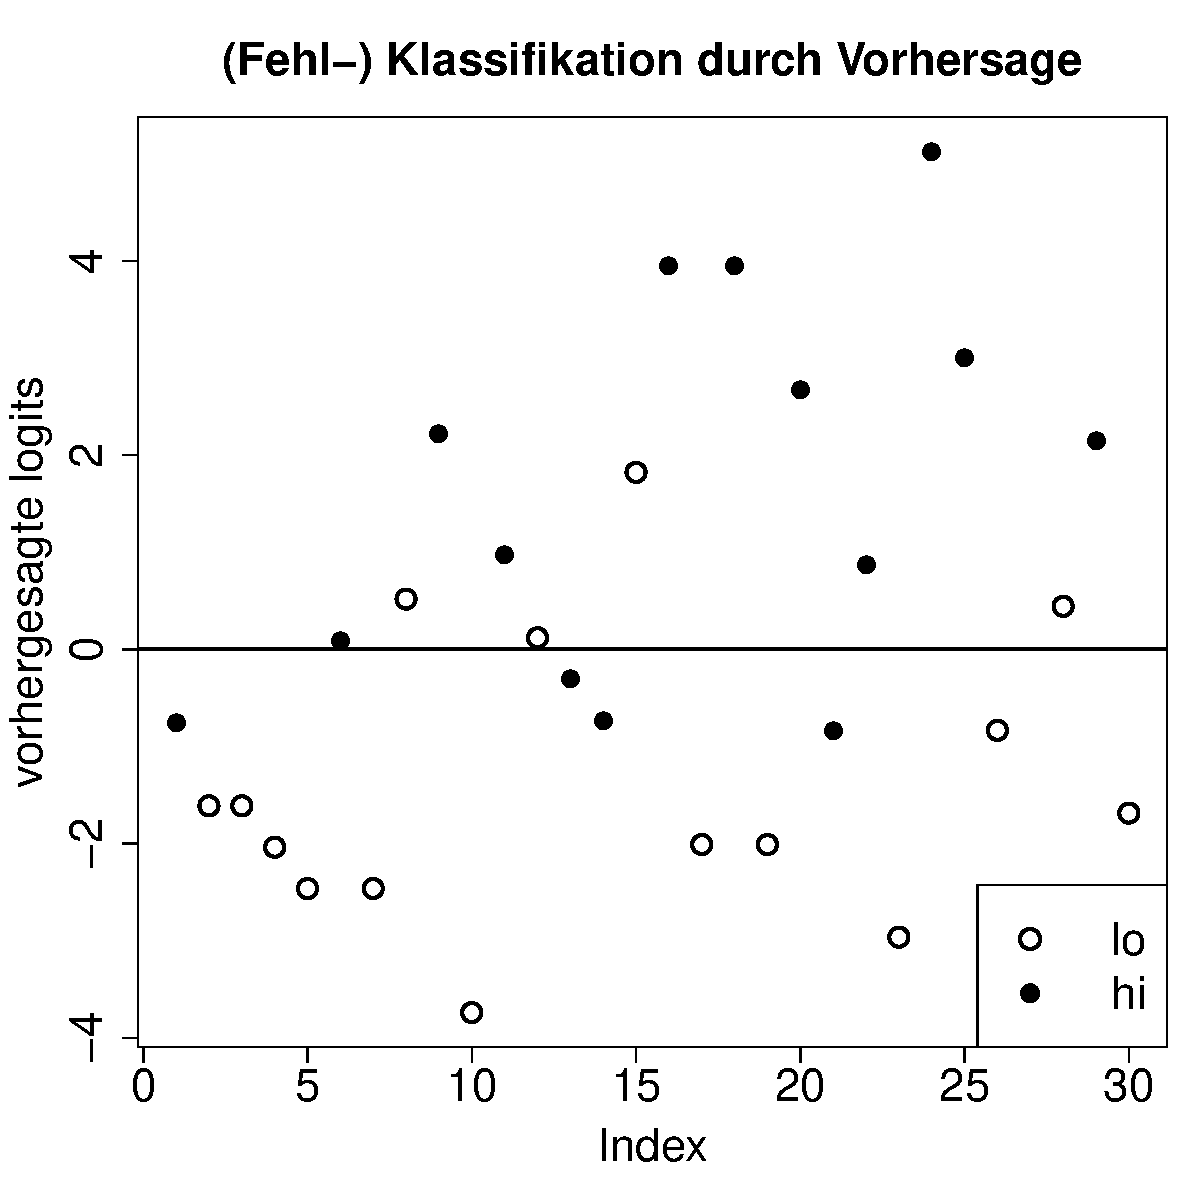
\includegraphics[width=8cm]{regrLog}
\vspace*{-1em}
\caption{Vorhersage und Daten einer logistischen Regression. Daten, die auf Basis der Vorhersage falsch klassifiziert würden, sind farblich hervorgehoben}
\label{fig:regrLog}
\end{figure}

An das Argument \lstinline!newdata! von \lstinline!predict()! kann zusätzlich ein Datensatz übergeben werden, der neue Daten für Variablen mit denselben Namen, und bei Faktoren zusätzlich denselben Stufen wie jene der ursprünglichen Prädiktoren enthält. Als Ergebnis erhält man die vorhergesagten Trefferwahrscheinlichkeiten für die neuen Prädiktorwerte (Abschn.\ \ref{sec:predict}).
\begin{lstlisting}
> Nnew  <- 3                          # Anzahl neuer Daten
> dfNew <- data.frame(DVpre=rnorm(Nnew, 20, sd=7),
+                        IV=factor(rep("SSRI", Nnew),
                                   levels=levels(dfAncova$IV)))

> predict(glmFit, newdata=dfNew, type="response")   # Vorhersage W'keit
          1           2           3
0.947324911 0.008185519 0.123296946
\end{lstlisting}

%%%%%%%%%%%%%%%%%%%%%%%%%%%%%%%%%%%%%%%%%%%%%%%%%%%%%%%%%%%%%%%%%%
%%%%%%%%%%%%%%%%%%%%%%%%%%%%%%%%%%%%%%%%%%%%%%%%%%%%%%%%%%%%%%%%%%
\subsection{Signifikanztests für Parameter und Modell}
\label{sec:regrLogTest}
%%%%%%%%%%%%%%%%%%%%%%%%%%%%%%%%%%%%%%%%%%%%%%%%%%%%%%%%%%%%%%%%%%
%%%%%%%%%%%%%%%%%%%%%%%%%%%%%%%%%%%%%%%%%%%%%%%%%%%%%%%%%%%%%%%%%%

Die geschätzten Gewichte $b$ lassen sich mit\index[func]{summary()@\lstinline{summary()}} \lstinline!summary(<<glm-Modell>>)! einzeln einem Wald-Signifikanztest unterziehen. In der Ausgabe finden sich dazu unter der Überschrift \lstinline!Coefficients! die Gewichte $b$ in der Spalte \lstinline!Estimate!, deren geschätzte Streuungen $\hat{\sigma}_{b}$ in der Spalte \lstinline!Std. Error! und die zugehörigen $z$-Werte $\frac{b}{\hat{\sigma}_{b}}$ in der Spalte \lstinline!z value!. Der Test setzt voraus, dass $z$ unter der Nullhypothese asymptotisch standardnormalverteilt ist. Die zugehörigen $p$-Werte stehen in der Spalte \lstinline!Pr(>|z|)!.
\begin{lstlisting}
> summary(glmFit)                    # Ausgabe gekürzt ...
Deviance Residuals:
    Min       1Q   Median       3Q      Max
-1.9865  -0.5629  -0.2372   0.4660   1.5455

Coefficients:
            Estimate Std. Error z value Pr(>|z|)
(Intercept)  -8.4230     2.9502  -2.855   0.0043 **
DVpre         0.4258     0.1553   2.742   0.0061 **
IVPlacebo     1.7306     1.2733   1.359   0.1741
IVWL          1.2027     1.2735   0.944   0.3450

(Dispersion parameter for binomial family taken to be 1)

    Null deviance: 41.455  on 29  degrees of freedom
Residual deviance: 24.409  on 26  degrees of freedom
AIC: 32.409

Number of Fisher Scoring iterations: 5
\end{lstlisting}

Die geschätzte Streuung der odds ratios $e^{b}$ erhalt man mit $\sqrt{\left(e^{b}\right)^{2} \cdot \hat{\sigma}^{2}_{b}}$.
\begin{lstlisting}
> OR    <- exp(coef(glmFit))      # odds ratios
> varB  <- diag(vcov(glmFit))     # Streuung geschätzte Koeffizienten
> (seOR <- sqrt(OR^2 * varB))[-1] # Streuung geschätzte odds ratios
       DVpre     IVPlacebo          IVWL
0.2377021539  7.1866998892  4.2397702028
\end{lstlisting}

Geeigneter als Wald-Tests sind oft Likelihood-Quotienten-Tests der Parameter, die auf der asymptotisch $\chi^{2}$-verteilten Devianz-Differenz zweier nested Modelle mit demselben Kriterium beruhen:\footnote{\label{ftn:HauckDonner}Bei Wald-Tests kann etwa das\index{Regression!Hauck-Donner-Phänomen} \emph{Hauck-Donner-Phänomen} auftreten: Bei starken Effekten (sehr große $\beta_{j}$) sind die berechneten Streuungen $\hat{\sigma}_{b}$ dann deutlich zu groß, wodurch Wald-Tests der Parameter fälschlicherweise nicht signifikant werden.} Der Prädiktorensatz des eingeschränkten Modells ist dabei vollständig im Prädiktorensatz des umfassenderen Modells enthalten, das zusätzlich noch weitere Prädiktoren berücksichtigt (Abschn.\ \ref{sec:regrCmp}). Solche Modellvergleiche können mit \lstinline!anova(<<fitR>>, <<fitU>>, test="Chisq")! durchgeführt werden, wobei \lstinline!<<fitR>>! das eingeschränkte und \lstinline!<<fitU>>! das umfassendere Modell ist. Zusätzlich lässt sich wie in der linearen Regression\index[func]{drop1()@\lstinline{drop1()}} \lstinline!drop1(<<glm-Modell>>, test="Chisq")! verwenden (Abschn.\ \ref{sec:regrCmp}).

Um das Gesamtmodell mit einem Likelihood-Quotienten-Test auf Signifikanz zu prüfen, muss somit\index[func]{anova()@\lstinline{anova()}} \lstinline!anova(<<0-Modell>>, <<glm-Modell>>, test="Chisq")! aufgerufen werden (Abschn.\ \ref{sec:regrCmp}). Der Test beruht auf dem Vergleich des angepassten Modells mit dem $0$-Modell, das nur eine Konstante als Prädiktor beinhaltet. Teststatistik ist die Devianz-Differenz beider Modelle mit der Differenz ihrer Freiheitsgrade als Anzahl der Freiheitsgrade der asymptotisch gültigen $\chi^{2}$-Verteilung.
\begin{lstlisting}
> glm0 <- update(glmFit, . ~ 1)                 # 0-Modell
> anova(glm0, glmFit, test="Chisq")             # Modellvergleich
Analysis of Deviance Table
Model 1: postFac ~ 1
Model 2: postFac ~ DVpre + IV
  Resid. Df Resid. Dev Df Deviance  Pr(>Chi)
1        29     41.455
2        26     24.409  3   17.047 0.0006912 ***

# manuelle Kontrolle
> chisqStat <- glmFit$null.deviance - deviance(glmFit)
> chisqDf   <- glmFit$df.null       - df.residual(glmFit)
> (pVal     <- pchisq(chisqStat, chisqDf, lower.tail=FALSE))
[1] 0.0006912397
\end{lstlisting}

Da der hier im Modell berücksichtigte Faktor \lstinline!IV! mit mehreren Parametern $\beta_{j}$ assoziiert ist, muss seine Signifikanz insgesamt über einen Modellvergleich gegen das vollständige Modell getestet werden.
\begin{lstlisting}
> glmPre <- update(glmFit, . ~ . - IV) # eingeschränktes Modell ohne IV
> anova(glmPre, glmFit, test="Chisq")  # Modellvergleich
Analysis of Deviance Table
Model 1: postFac ~ DVpre
Model 2: postFac ~ DVpre + IV
  Resid. Df Resid. Dev Df Deviance Pr(>Chi)
1        28     26.566
2        26     24.409  2   2.1572   0.3401
\end{lstlisting}

Analog erfolgt für Quadratsummen vom Typ I (Abschn.\ \ref{sec:ssTypes}) der Test des kontinuierlichen Prädiktors \lstinline!DVpre! als Vergleich des Modells nur mit \lstinline!DVpre! mit dem $0$-Modell.
\begin{lstlisting}
> anova(glm0, glmPre, test="Chisq")             # Modellvergleich
Analysis of Deviance Table
Model 1: postFac ~ 1
Model 2: postFac ~ DVpre
  Resid. Df Resid. Dev Df Deviance Pr(>Chi)
1        29     41.455
2        28     26.566  1    14.89 0.000114 ***
\end{lstlisting}

%%%%%%%%%%%%%%%%%%%%%%%%%%%%%%%%%%%%%%%%%%%%%%%%%%%%%%%%%%%%%%%%%%
%%%%%%%%%%%%%%%%%%%%%%%%%%%%%%%%%%%%%%%%%%%%%%%%%%%%%%%%%%%%%%%%%%
\subsection{Andere Link-Funktionen}
\label{sec:glmOtherLink}
%%%%%%%%%%%%%%%%%%%%%%%%%%%%%%%%%%%%%%%%%%%%%%%%%%%%%%%%%%%%%%%%%%
%%%%%%%%%%%%%%%%%%%%%%%%%%%%%%%%%%%%%%%%%%%%%%%%%%%%%%%%%%%%%%%%%%

Eine meist zu ähnlichen Ergebnissen führende Alternative zur logistischen Regression ist die\index{Regression!Probit-Regression}\index{Probit-Regression|see{Regression}} Probit-Regression. Sie verwendet als Link-Funktion $\Phi^{-1}(\cdot)$, die Umkehrfunktion der Verteilungsfunktion $\Phi(\cdot)$ der Standardnormalverteilung, wofür das Argument \lstinline!family! von \lstinline!glm()! auf \lstinline!binomial(link="probit")! zu setzen ist. Hier ist also $P = \Phi(\bm{X} \bm{\beta})$. Eine weitere Link-Funktion, die mit bedingter Binomialverteilung von $Y$ kombiniert werden kann, ist die komplementäre log-log-Funktion $\ln(-\ln(1-P))$. Man erhält sie mit \lstinline!binomial(link="cloglog")!. Mit ihrer Umkehrfunktion, der Verteilungsfunktion der Gumbel-Verteilung, gilt $P = 1 - \exp(-\exp(\bm{X} \bm{\beta}))$ -- dabei steht $\exp(\cdot)$ aus typografischen Gründen für $\euler^{(\cdot)}$.

Mitunter streuen empirische Residuen stärker, als dies bei bedingter Binomialverteilung mit der Varianz $n_{i} \, P \, (1-P)$ zu erwarten wäre (\emph{overdispersion}). Ein Hinweis auf overdispersion ist ein Verhältnis von Residual-Devianz zu Residual-Freiheitsgraden, das deutlich größer als $1$ ist. Die modellbasierten Streuungsschätzungen unterschätzen dann die wahre Streuung, was zu liberale Signifikanztests der Parameter zur Folge hat. Eine mögliche Ursache für overdispersion ist ein unvollständiges Vorhersagemodell, das tatsächlich relevante Prädiktoren nicht berücksichtigt. Bei overdispersion kann ein Binomial-ähnliches Modell verwendet werden, das einen zusätzlichen, aus den Daten zu schätzenden Streuungsparameter $\phi$ besitzt, mit dem für die bedingte Varianz $\sigma^{2} = \phi \, n_{i} \, P \, (1-P)$ gilt: Hierfür ist \lstinline!family! auf \lstinline!quasibinomial(link="logit")! zu setzen. Die Parameterschätzungen $b$ sind dann identisch zur logistischen Regression, die geschätzten Streuungen $\hat{\sigma}_{b}$ jedoch unterschiedlich, was zu anderen Ergebnissen der inferenzstatistischen Tests führt.

Da die bedingte Verteilung der Daten in der quasi-binomial Familie bis auf Erwartungswert und Varianz unspezifiziert bleibt, ist die Likelihood-Funktion der Daten für gegebene Parameter unbekannt. Trotzdem kann jedoch die IWLS-Methode Parameter schätzen (Abschn.\ \ref{sec:glmConvergence}), wobei dann alle likelihood-basierten Kennwerte wie AIC oder pseudo-$R^{2}$ nicht zur Verfügung stehen. Durch die Schätzung des Streuungs-Parameters sind die Wald-Teststatistiken keine $z$-, sondern $t$-Werte. Analog sollten Modellvergleiche mit einem $F$-Test über das Argument \lstinline!anova(..., test="F")! durchgeführt werden statt über einen $\chi^{2}$-Test wie bei bekannter Varianz.

Den Spezialfall einer linearen Regression erhält man mit \lstinline!gaussian(link="identity")!. Die Maximum-Likelihood-Schätzungen der Parameter stimmen dann mit den durch \lstinline!lm()! ermittelten Schätzern der linearen Regression überein.

%%%%%%%%%%%%%%%%%%%%%%%%%%%%%%%%%%%%%%%%%%%%%%%%%%%%%%%%%%%%%%%%%%
%%%%%%%%%%%%%%%%%%%%%%%%%%%%%%%%%%%%%%%%%%%%%%%%%%%%%%%%%%%%%%%%%%
\subsection{Mögliche Probleme bei der Modellanpassung}
\label{sec:glmConvergence}
%%%%%%%%%%%%%%%%%%%%%%%%%%%%%%%%%%%%%%%%%%%%%%%%%%%%%%%%%%%%%%%%%%
%%%%%%%%%%%%%%%%%%%%%%%%%%%%%%%%%%%%%%%%%%%%%%%%%%%%%%%%%%%%%%%%%%

\index{Regression!logistische!Konvergenz}
Die Maximum-Likelihood-Schätzung der Parameter ist nicht in geschlossener Form darstellbar, sondern muss mit einem numerischen Optimierungsverfahren gefunden werden -- typischerweise über die IWLS-Methode (\emph{iterative weighted least squares}). Diese numerische Suche nach dem Maximum der Likelihood-Funktion kann in seltenen Fällen fehlschlagen, auch wenn es ein eindeutiges Maximum gibt. Ursache einer nicht konvergierenden Suche ist häufig, dass sie an einem Punkt von Schätzungen beginnt, der zu weit vom tatsächlichen Maximum entfernt ist.

Konvergenz-Probleme können durch Warnmeldungen angezeigt werden (etwa \emph{algorithm did not converge}), sich in sehr großen Schätzungen bei gleichzeitig sehr großen Standardfehlern äußern oder in einer Residual-Devianz, die größer als die Devianz des Null-Modells ist. In diesen Fällen ist das Ergebnis von \lstinline!glm()! nicht gültig. Ob Konvergenz erreicht wurde, speichert die von \lstinline!glm()! zurückgegebene Liste in der Komponente \lstinline!converged!.

Um die Konvergenz der Suche zu begünstigen, lässt sich über das Argument \lstinline!start! manuell ein Vektor von Start-Werten für alle Parameter vorgeben. Eine Strategie für ihre Wahl besteht darin, eine gewöhnliche lineare Regression der logit-transformierten Variable $Y$ durchzuführen und deren Parameter-Schätzungen zu wählen. Konvergenzprobleme lassen sich u.\,U.\ auch über eine höhere maximale Anzahl von Suchschritten beheben, die in der Voreinstellung $25$ beträgt und so geändert werden kann:
\begin{lstlisting}
glm(..., control=glm.control(maxit=<<Anzahl>>))
\end{lstlisting}

\index{Regression!logistische!Konvergenz!Separierbarkeit}
Die Maximum-Likelihood-Schätzung der Parameter setzt voraus, dass keine (quasi-) vollständige Separierbarkeit von Prädiktoren durch die Kategorien von $Y$ vorliegt \cite{Allison2008, Allison2003}. Dies ist der Fall, wenn $Y$ stellenweise perfekt aus einer Linearkombination der Prädiktoren vorhersagbar ist. Das zugehörige geschätzte odds ratio $\euler^{\hat{\beta}_{j}}$ müsste dann $\infty$ sein. Eine mögliche Ursache sind schwach besetzte Gruppen bei kategorialen Kovariaten. Ein Symptom für (quasi-) vollständige Separierbarkeit ist die Warnmeldung, dass geschätzte Trefferwahrscheinlichkeiten von $0$ bzw.\ $1$ aufgetreten sind. Ein weiteres Symptom für Separierbarkeit sind sehr große Parameterschätzungen, die mit großen Standardfehlern assoziiert sind und daher im Wald-Test kleine $z$-Werte liefern.

In diesen Fällen kann auf Bayes-Methoden mit schwach informativer A-priori-Verteilung (etwa mit dem Paket \lstinline!rstanarm!\index[pack]{rstanarm@\lstinline{rstanarm}}) oder auf penalisierte Verfahren ausgewichen werden. Dazu zählt die logistische Regression mit Firth-Korrektur, die im Paket \index[pack]{logistf@\lstinline{logistf}} \lstinline!logistf! \cite{Heinze2013a} umgesetzt wird (Abschn.\ \ref{sec:lmPen}). Eine andere Möglichkeit besteht darin, Kategorien in relevanten Prädiktorvariablen zusammenzufassen.

%%%%%%%%%%%%%%%%%%%%%%%%%%%%%%%%%%%%%%%%%%%%%%%%%%%%%%%%%%%%%%%%%%
%%%%%%%%%%%%%%%%%%%%%%%%%%%%%%%%%%%%%%%%%%%%%%%%%%%%%%%%%%%%%%%%%%
\section{Ordinale Regression}
\label{sec:regrOrd}
%%%%%%%%%%%%%%%%%%%%%%%%%%%%%%%%%%%%%%%%%%%%%%%%%%%%%%%%%%%%%%%%%%
%%%%%%%%%%%%%%%%%%%%%%%%%%%%%%%%%%%%%%%%%%%%%%%%%%%%%%%%%%%%%%%%%%

\index{Regression!ordinale}
\index{Ordinale Regression|see{Regression}}
In der ordinalen Regression soll eine kategoriale Variable $Y$ mit $k$ geordneten Kategorien $1, \dots, g, \dots, k$ mit $p$ Prädiktoren $X_{j}$ vorhergesagt werden. Dazu führt man die Situation auf jene der logistischen Regression zurück (Abschn.\ \ref{sec:regrLog}), indem man zunächst $k-1$ dichotome Kategorisierungen $Y \geq g$ vs.\ $Y < g$ mit $g = 2, \ldots, k$ vornimmt. Mit diesen dichotomen Kategorisierungen lassen sich nun $k-1$ \emph{kumulative} Logits bilden:
\begin{equation*}
\text{logit}(P(Y \geq g)) = \ln \frac{P(Y \geq g)}{1 - P(Y \geq g)} = \ln \frac{P(Y=g) + \dots + P(Y=k)}{P(Y=1) + \dots + P(Y=g-1)}
\end{equation*}

Die $k-1$ kumulativen Logits geben jeweils die logarithmierte Chance dafür an, dass $Y$ mindestens die Kategorie $g$ erreicht. Sie werden in $k-1$ separaten logistischen Regressionen mit dem Modell $\text{logit}(P(Y \geq g)) = \beta_{0_{g}} + \beta_{1} X_{1} + \dots + \beta_{p} X_{p}$ linear vorhergesagt ($g = 2, \ldots, k$). Die Parameterschätzungen erfolgen dabei für alle Regressionen simultan mit der Nebenbedingung, dass die Menge der $\beta_{j}$ für alle $g$ identisch ist und $\beta_{0_{2}} > \dots > \beta_{0_{k}}$ gilt. In diesem Modell führt ein höherer Prädiktorwert $X_{j}$ bei positivem $\beta_{j}$ zu einer höheren Chance, dass eine höhere Kategorie von $Y$ erreicht wird.\footnote{Andere Formulierungen des Modells sind möglich. So legt etwa \index{SPSS} SPSS das Modell $\text{logit}(P(Y \leq g)) = \beta_{0_{g}} - (\beta_{1} X_{1} + \dots + \beta_{p} X_{p})$  mit der Nebenbedingung $\beta_{0_{1}} < \dots < \beta_{0_{k-1}}$ zugrunde, das jedoch nur zu umgedrehten Vorzeichen der Schätzungen für die $\beta_{0_{g}}$ führt. Mit derselben Nebenbedingung ließe sich das Modell auch als $\text{logit}(P(Y \leq g)) = \beta_{0_{g}} + \beta_{1} X_{1} + \dots + \beta_{p} X_{p}$ formulieren. In diesem Modell führt ein höherer Prädiktorwert $X_{j}$ bei positivem $\beta_{j}$ zu einer höheren Chance, dass eine \emph{niedrigere} Kategorie von $Y$ erreicht wird. Entsprechend haben hier die Schätzungen für alle Parameter umgekehrte Vorzeichen.}

Kern des Modells ist die Annahme, dass eine additive Erhöhung des Prädiktorwerts $X_{j}$ um den Wert $c$ dazu führt, dass die Chance für eine höhere Kategorie unabhängig von $g$ um den festen Faktor $\euler^{\beta_{j} c}$ wächst: $\frac{P(Y \geq g | X_{j}+c)}{P(Y < g | X_{j}+c)} = \euler^{\beta_{j} c} \, \frac{P(Y \geq g | X_{j})}{P(Y < g | X_{j})}$. Aus diesem Grund heißt es auch \emph{proportional odds} Modell. Wie in der logistischen Regression ist damit $\euler^{\beta_{j}}$ das odds ratio, also der Faktor, um den der vorhergesagte Wettquotient zunimmt, wenn $X_{j}$ um eine Einheit wächst.\footnote{\label{ftn:ordLogits}Alternative proportional odds Modelle sind zum einen mit \emph{adjacent category} Logits $\ln \frac{P(Y=g)}{P(Y=g-1)}$ möglich, zum anderen mit \emph{continuation ratio} (\emph{sequentiellen}) Logits $\ln \frac{P(Y=g)}{P(Y<g)}$.}

Wegen $P(Y=g) = P(Y \geq g) - P(Y \geq g+1)$ hat die Link-Funktion sowie ihre Umkehrfunktion hier eine zusammengesetzte Form. Mit der logistischen Funktion als Umkehrfunktion der Logit-Funktion sind die theoretischen Parameter $P(Y=g)$ identifizierbar als:
\begin{equation*}
P(Y=g) = \frac{\euler^{\beta_{0_{g}} + \beta_{1} X_{1} + \dots + \beta_{p} X_{p}}}{1 + \euler^{\beta_{0_{g}} + \beta_{1} X_{1} + \dots + \beta_{p} X_{p}}} - \frac{e^{\beta_{0_{g+1}} + \beta_{1} X_{1} + \dots + \beta_{p} X_{p}}}{1 + \euler^{\beta_{0_{g+1}} + \beta_{1} X_{1} + \dots + \beta_{p} X_{p}}}
\end{equation*}

Die Modellannahmen lassen sich grafisch veranschaulichen (Abb.\ \ref{fig:regrOrdMod}): Bei einem Prädiktor $X$ sind die $k-1$ kumulativen Logits lineare Funktionen von $X$ mit derselben Steigung und geordneten $y$-Achsenabschnitten. Die Wahrscheinlichkeit dafür, dass $Y$ mindestens die Kategorie $g = 2, \ldots, k$ erreicht, ergibt sich aus $k-1$ parallelen logistischen Funktionen mit der horizontalen Verschiebung $\frac{\beta_{0_{g+1}} - \beta_{0_{g}}}{\beta_{1}}$, d.\,h.\ $P(Y \geq g+1|X) = P(Y \geq g | X - \frac{\beta_{0_{g+1}} - \beta_{0_{g}}}{\beta_{1}})$.

\begin{figure}[ht]
\centering
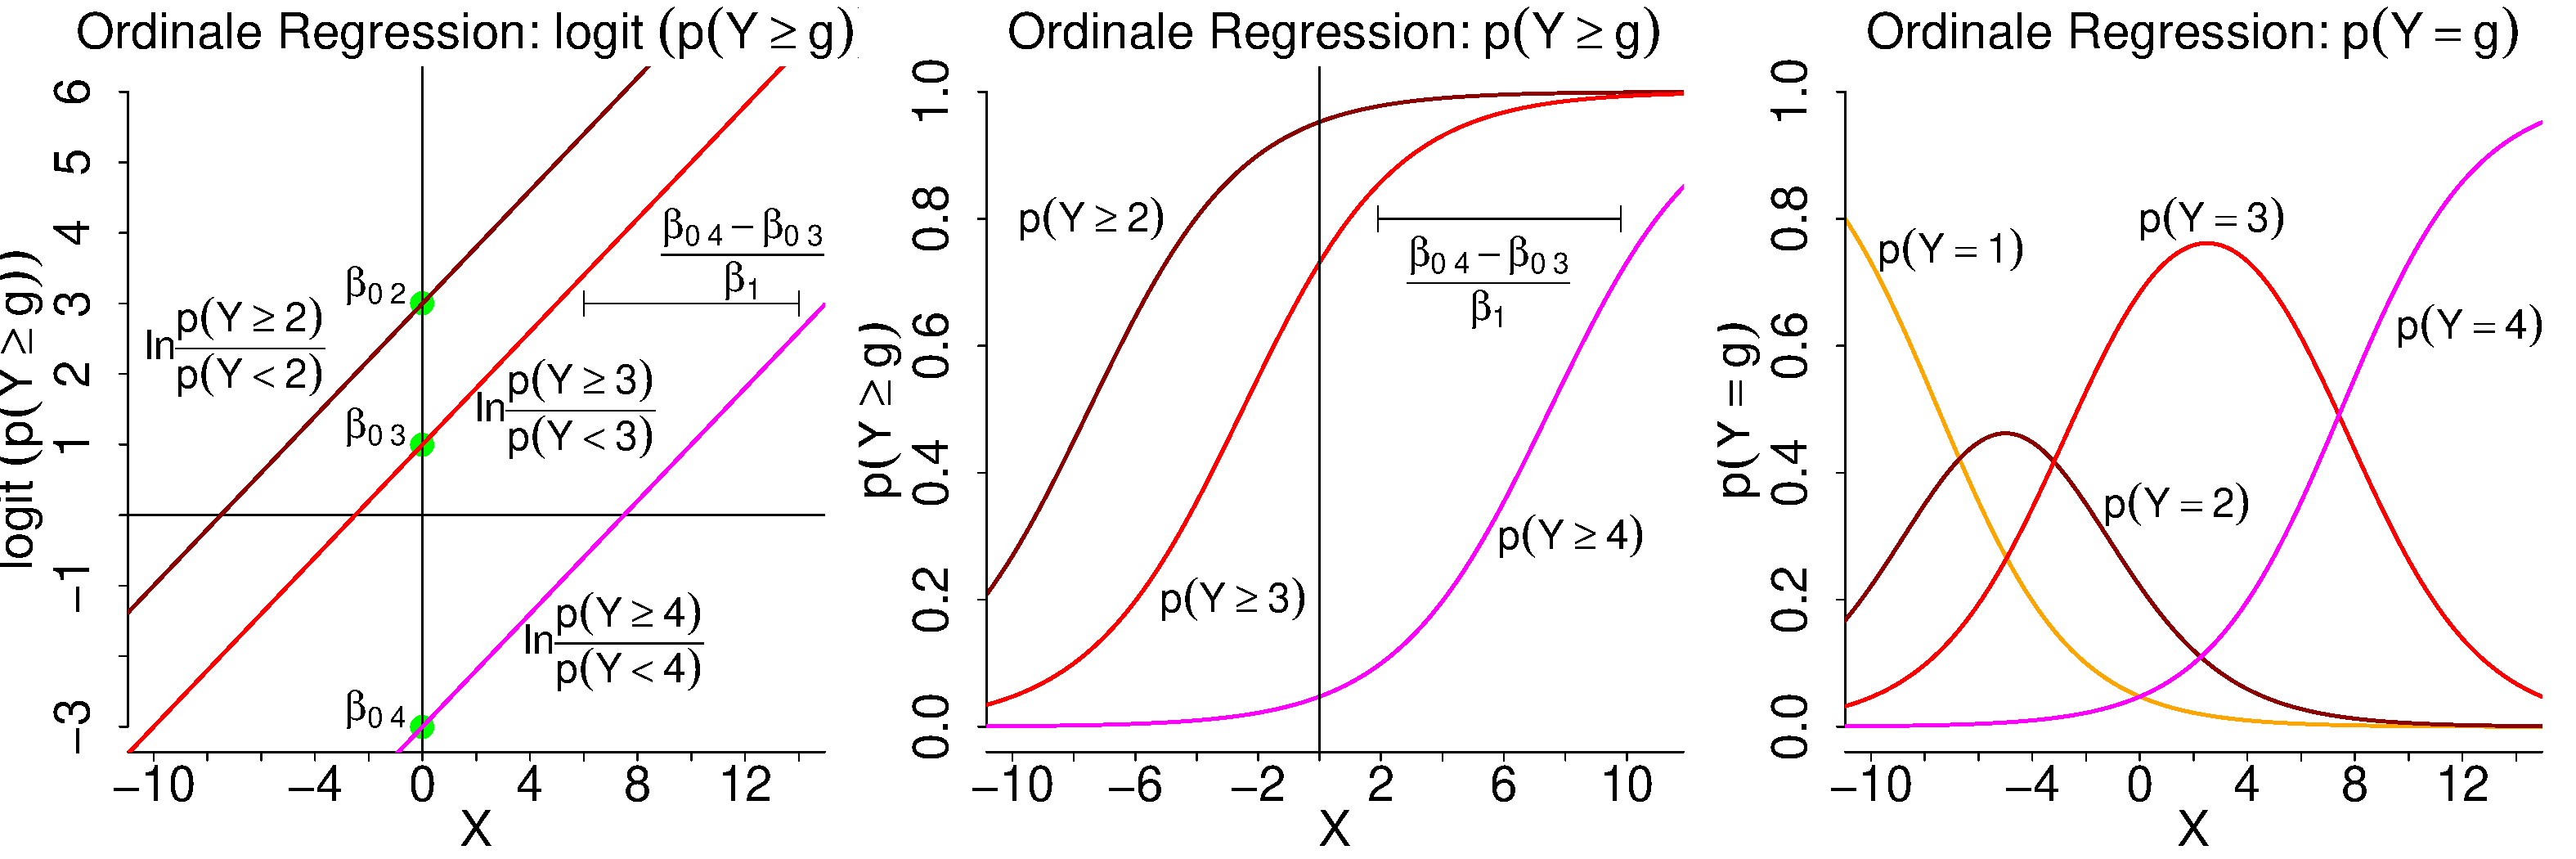
\includegraphics[width=12.5cm]{regrOrdMod}
\vspace*{-0.5em}
\caption{Modellannahmen der ordinalen Regression bei einem Prädiktor und $4$ Kategorien des Kriteriums $Y$: Linearität der $3$ kumulativen Logits mit identischer Steigung; parallel verschobene logistische Funktionen jeweils für die Wahrscheinlichkeit, mindestens Kategorie $g$ zu erreichen; stochastisch geordnete Funktionen für die Wahrscheinlichkeit von $Y=g$.}
\label{fig:regrOrdMod}
\end{figure}

%%%%%%%%%%%%%%%%%%%%%%%%%%%%%%%%%%%%%%%%%%%%%%%%%%%%%%%%%%%%%%%%%%
%%%%%%%%%%%%%%%%%%%%%%%%%%%%%%%%%%%%%%%%%%%%%%%%%%%%%%%%%%%%%%%%%%
\subsection{Modellanpassung}
\label{sec:regrOrdFit}
%%%%%%%%%%%%%%%%%%%%%%%%%%%%%%%%%%%%%%%%%%%%%%%%%%%%%%%%%%%%%%%%%%
%%%%%%%%%%%%%%%%%%%%%%%%%%%%%%%%%%%%%%%%%%%%%%%%%%%%%%%%%%%%%%%%%%

Das proportional odds Modell mit kumulativen Logits kann mit\index[func]{vglm()@\lstinline{vglm()}} \lstinline!vglm()! aus dem Paket\index[pack]{VGAM@\lstinline{VGAM}|textbf} \lstinline!VGAM! \cite{Yee2010} angepasst werden. Diese Funktion hat gegenüber anderen, später ebenfalls erwähnten Funktionen den Vorteil, dass sie sich für alle in diesem Kapitel behandelten Modelle eignet und damit eine konsistente Herangehensweise an verwandte Fragestellungen ermöglicht.
\begin{lstlisting}
vglm(<<Modellformel>>, family=<<Modell>>, data=<<Datensatz>>)
\end{lstlisting}

Die Modellformel ist wie bei \lstinline!glm()! zu formulieren, ihre linke Seite muss ein geordneter Faktor sein (Abschn.\ \ref{sec:facOrder}). Für das proportional odds Modell ist \lstinline!family=propodds! zu setzen.\footnote{Mit \lstinline!vglm()! ist es möglich, auch die proportional odds Modelle mit adjacent category Logits bzw.\ continuation ratio Logits anzupassen (Abschn.\ \ref{sec:regrOrd}, Fußnote \ref{ftn:ordLogits}). Dazu ist \lstinline!family! auf \lstinline!acat(parallel=TRUE)! bzw.\ auf \lstinline!sratio(parallel=TRUE)! zu setzen. Eine weitere Option für \lstinline!acat()! bzw.\ \lstinline!sratio()! ist dabei das Argument \lstinline!reverse!, das die Vergleichsrichtung dieser Logits bzgl.\ der Stufen von $Y$ kontrolliert und auf \lstinline!TRUE! oder \lstinline!FALSE! gesetzt werden kann.} Schließlich benötigt \lstinline!data! den Datensatz mit den Variablen aus der Modellformel.

Als Beispiel soll eine Variable mit $k=4$ geordneten Kategorien anhand von $p=2$ Prädiktoren vorhergesagt werden. Die kategoriale Zielgröße soll sich dabei aus der Diskretisierung einer kontinuierlichen Variable ergeben.
\begin{lstlisting}
> N     <- 100
> X1    <- rnorm(N, 175, 7)                       # Prädiktor 1
> X2    <- rnorm(N,  30, 8)                       # Prädiktor 2
> Ycont <- 0.5*X1 - 0.3*X2 + 10 + rnorm(N, 0, 6)  # kontinuierlich

# geordneter Faktor aus Diskretisierung der kontinuierlichen Zielgröße
> Yord <- cut(Ycont, breaks=quantile(Ycont), include.lowest=TRUE,
+             labels=c("--", "-", "+", "++"), ordered=TRUE)

# zugehöriger ungeordneter Faktor für spätere Auswertungen
> Ycateg <- factor(Yord, ordered=FALSE)
> dfOrd  <- data.frame(X1, X2, Yord, Ycateg)      # Datensatz

> library(VGAM)                                   # für vglm()
> vglmFit <- vglm(Yord ~ X1 + X2, family=propodds, data=dfOrd)
\end{lstlisting}

Die $k-1$ Schätzungen der Parameter $\beta_{0_{g}}$ sowie die $p$ Schätzungen der Parameter $\beta_{j}$ können mit \lstinline!coef(<<vglm-Modell>>)! extrahiert werden. Die $b_{j}$ sind wie in der logistischen Regression zu exponenzieren, um die geschätzten odds ratios zu erhalten (Abschn.\ \ref{sec:glmFit}): $\euler^{b_{j}}$ gibt an, um welchen Faktor die vorhergesagte Chance wächst, eine höhere Kategorie zu erreichen, wenn sich $X_{j}$ um eine Einheit erhöht. Die proportional odds Annahme bedeutet, dass sich die Wechselchance bei allen Kategorien im selben Maße ändert.
\begin{lstlisting}
> exp(coef(vglmFit))                              # odds ratios
(Intercept):1 (Intercept):2 (Intercept):3            X1            X2
 3.554552e-11  9.225479e-12  2.195724e-12  1.170903e+00  9.355142e-01
\end{lstlisting}

%%%%%%%%%%%%%%%%%%%%%%%%%%%%%%%%%%%%%%%%%%%%%%%%%%%%%%%%%%%%%%%%%%
%%%%%%%%%%%%%%%%%%%%%%%%%%%%%%%%%%%%%%%%%%%%%%%%%%%%%%%%%%%%%%%%%%
\subsection{Anpassungsgüte}
%%%%%%%%%%%%%%%%%%%%%%%%%%%%%%%%%%%%%%%%%%%%%%%%%%%%%%%%%%%%%%%%%%
%%%%%%%%%%%%%%%%%%%%%%%%%%%%%%%%%%%%%%%%%%%%%%%%%%%%%%%%%%%%%%%%%%

Wie in der logistischen Regression dienen verschiedene Maße als Anhaltspunkte zur Anpassungsgüte des Modells (Abschn.\ \ref{sec:regrLogRsq}). Dazu zählt die Devianz ebenso wie das Informationskriterium AIC sowie die pseudo-$R^{2}$ Kennwerte.\footnote{Weitere Gütemaße der Modellanpassung erzeugt \lstinline!orm()! aus dem Paket \lstinline!rms! (Abschn.\ \ref{sec:regrLogRsq}, Fußnote \ref{ftn:rmsLrm}).}
\begin{lstlisting}
> deviance(vglmFit)             # Devianz
[1] 244.1915

> AIC(vglmFit)                  # Informationskriterium AIC
[1] 254.1915

> library(DescTools)            # für PseudoR2()
> PseudoR2(vglmFit, which="Nagelkerke")
Nagelkerke 
0.3003312
\end{lstlisting}

Für potentiell auftretende Probleme bei der Modellanpassung s.\ Abschn.\ \ref{sec:glmConvergence}.

%%%%%%%%%%%%%%%%%%%%%%%%%%%%%%%%%%%%%%%%%%%%%%%%%%%%%%%%%%%%%%%%%%
%%%%%%%%%%%%%%%%%%%%%%%%%%%%%%%%%%%%%%%%%%%%%%%%%%%%%%%%%%%%%%%%%%
\subsection{Signifikanztests für Parameter und Modell}
%%%%%%%%%%%%%%%%%%%%%%%%%%%%%%%%%%%%%%%%%%%%%%%%%%%%%%%%%%%%%%%%%%
%%%%%%%%%%%%%%%%%%%%%%%%%%%%%%%%%%%%%%%%%%%%%%%%%%%%%%%%%%%%%%%%%%

Mit \lstinline!summary(<<vglm-Modell>>)! werden neben den Parameterschätzungen $b$ auch ihre geschätzten Streuungen $\hat{\sigma}_{b}$ sowie die zugehörigen $z$-Werte $\frac{b}{\hat{\sigma}_{b}}$ berechnet. Mit der Annahme, dass $z$ unter der Nullhypothese asymptotisch standardnormalverteilt ist, stehen die zweiseitigen $p$-Werte in der Spalte \lstinline!Pr(>|z|)!. Die genannten Werte lassen sich mit \lstinline!coef(summary(<<vglm-Modell>>))! extrahieren. Profile-Likelihood Konfidenzintervalle erzeugt\index[func]{confint()@\lstinline{confint()}} \lstinline!confint(<<vglm-Modell>>, method="profile")!.
\begin{lstlisting}
> sumOrd   <- summary(vglmFit)
> (coefOrd <- coef(sumOrd))
                  Estimate Std. Error   z value     Pr(>|z|)
(Intercept):1 -24.06020695 5.82571121 -4.130003 3.627579e-05
(Intercept):2 -25.40905205 5.87912090 -4.321914 1.546818e-05
(Intercept):3 -26.84450928 5.94234461 -4.517495 6.257564e-06
X1              0.15777487 0.03385696  4.660042 3.161443e-06
X2             -0.06665895 0.02499298 -2.667107 7.650735e-03

> confint(vglmFit, method="profile")
                     2.5 %       97.5 %
(Intercept):1 -35.73662098 -12.97698381
(Intercept):2 -37.20085293 -14.23533935
(Intercept):3 -38.78768133 -15.55313940
X1              0.09392565   0.22569264
X2             -0.11661985  -0.01890649
\end{lstlisting}

Eine oft geeignetere Alternative zu Wald-Tests sind Likelihood-Quotienten-Tests eines umfassenderen Modells \lstinline!<<fitU>>! gegen ein eingeschränktes Modell \lstinline!<<fitR>>! mit\index[func]{anova()@\lstinline{anova()}} \lstinline!anova(<<fitR>>, <<fitU>>, type="I")! aus dem Paket\index[pack]{VGAM@\lstinline{VGAM}} \lstinline!VGAM! (Abschn.\ \ref{sec:regrLogTest}). Der $p$-Wert steht in der Ausgabe in der Spalte \lstinline!Pr(>Chi)!.
\begin{lstlisting}
# eingeschränktes Modell ohne Prädiktor X2
> vglmR <- vglm(Yord ~ X1, family=propodds, data=dfOrd)
> anova(vglmR, vglmFit, type="I")         # Likelihood-Quotienten-Test
Analysis of Deviance Table
Model 1: Yord ~ X1
Model 2: Yord ~ X1 + X2
  Resid. Df Resid. Dev Df Deviance Pr(>Chi)   
1       296     251.75                        
2       295     244.19  1   7.5568 0.005978 **
\end{lstlisting}

Auf diese Weise lässt sich auch das Gesamtmodell gegen das $0$-Modell ohne Prädiktoren $X_{j}$ testen.
\begin{lstlisting}
# Null-Modell ohne Prädiktoren
> vglm0 <- vglm(Yord ~ 1,  family=propodds, data=dfOrd)
> anova(vglm0, vglmFit, type="I")         # Test des Gesamtmodells
Analysis of Deviance Table
Model 1: Yord ~ 1
Model 2: Yord ~ X1 + X2
  Resid. Df Resid. Dev Df Deviance Pr(>Chi)    
1       297     277.26                         
2       295     244.19  2   33.067  6.6e-08 ***
\end{lstlisting}

Ohne die proportional odds Annahme, dass die Menge der $\beta_{j}$ in allen $k-1$ separaten Regressionen der kumulativen Logits identisch ist, erhält man ein umfassenderes Modell. Die Parameter $\beta_{j_{g}}$ sind dann von $g$ abhängig, die linearen Funktionen für die Logits also nicht mehr parallel (Abb.\ \ref{fig:regrOrdMod}). Dieses Modell lässt sich ebenfalls mit \lstinline!vglm()! anpassen, indem man \lstinline!family! auf \lstinline!cumulative(parallel=FALSE)! setzt. Der Likelihood-Quotienten-Test des umfassenderen Modells gegen das eingeschränkte Modell mit proportional odds Annahme erfolgt wieder mit \lstinline!anova()!. Fällt der Test signifikant aus, ist dies ein Hinweis darauf, dass die Daten gegen die proportional odds Annahme sprechen.
\begin{lstlisting}
# eingeschränktes Modell - äquivalent zu vglm(..., family=propodds)
> vglmP <- vglm(Yord ~ X1 + X2, family=cumulative(parallel=TRUE,
+               reverse=TRUE), data=dfOrd)

# umfassenderes Modell ohne proportional odds Annahme
> vglmNP <- vglm(Yord ~ X1 + X2, family=cumulative(parallel=FALSE,
+                reverse=TRUE), data=dfOrd)

> anova(vglmNP, vglmP, type="I")        # Likelihood-Quotienten-Test
Analysis of Deviance Table
Model 1: Yord ~ X1 + X2
Model 2: Yord ~ X1 + X2
  Resid. Df Resid. Dev Df Deviance Pr(>Chi)
1       291     239.79                     
2       295     244.19 -4  -4.4033   0.3542
\end{lstlisting}

%%%%%%%%%%%%%%%%%%%%%%%%%%%%%%%%%%%%%%%%%%%%%%%%%%%%%%%%%%%%%%%%%%
%%%%%%%%%%%%%%%%%%%%%%%%%%%%%%%%%%%%%%%%%%%%%%%%%%%%%%%%%%%%%%%%%%
\subsection{Vorhersage, Klassifikation und Anwendung auf neue Daten}
%%%%%%%%%%%%%%%%%%%%%%%%%%%%%%%%%%%%%%%%%%%%%%%%%%%%%%%%%%%%%%%%%%
%%%%%%%%%%%%%%%%%%%%%%%%%%%%%%%%%%%%%%%%%%%%%%%%%%%%%%%%%%%%%%%%%%

Die vorhergesagten Kategorienwahrscheinlichkeiten $\hat{P}(Y = g)$ erhält man wie in der logistischen Regression mit\index[func]{predict()@\lstinline{predict()}} \lstinline!predict(<<vglm-Modell>>, type="response")!. Die ausgegebene Matrix enthält für jede Beobachtung (Zeilen) die vorhergesagte Wahrscheinlichkeit für jede Kategorie (Spalten).
\begin{lstlisting}
> PhatCateg <- predict(vglmFit, type="response")
> head(PhatCateg, n=3)
    Yord=--    Yord=-    Yord=+    Yord=++
1 0.1433775 0.2486796 0.3383702 0.26957271
2 0.2785688 0.3194630 0.2640555 0.13791266
3 0.5278107 0.2837526 0.1360684 0.05236823
\end{lstlisting}

Die vorhergesagten Kategorien selbst lassen sich aus den vorhergesagten Kategorienwahrscheinlichkeiten bestimmen, indem pro Beobachtung die Kategorie mit der maximalen vorhergesagten Wahrscheinlichkeit herangezogen wird. Das zeilenweise Maximum einer Matrix gibt\index[func]{max.col()@\lstinline{max.col()}} \lstinline!max.col(<<Matrix>>)! aus.
\begin{lstlisting}
> categHat <- levels(dfOrd$Yord)[max.col(PhatCateg)]
> head(categHat)
[1] "+"  "-"  "--"  "+"  "-"  "+"
\end{lstlisting}

Die Kontingenztafel tatsächlicher und vorhergesagter Kategorien eignet sich als Grundlage für die Berechnung von Übereinstimmungsmaßen wie der Rate der korrekten Klassifikation. Hier ist darauf zu achten, dass die Kategorien identisch geordnet sind.
\begin{lstlisting}
# Faktor mit gleich geordneten Kategorien
> facHat <- factor(categHat, levels=levels(dfOrd$Yord))

# Kontingenztafel tatsächlicher und vorhergesagter Kategorien
> cTab <- table(dfOrd$Yord, facHat, dnn=c("Yord", "facHat"))
> addmargins(cTab)                      # Randsummen hinzufügen
     facHat
Yord   --   -   +  ++ Sum
  --   10   7   7   1  25
  -    10   7   4   4  25
  +     5   7   7   6  25
  ++    0   2   9  14  25
  Sum  25  23  27  25 100

> (CCR <- sum(diag(cTab)) / sum(cTab))  # Rate der korrekten Klass.
[1] 0.38
\end{lstlisting}

An das Argument \lstinline!newdata! von \lstinline!predict()! kann zusätzlich ein Datensatz übergeben werden, der neue Daten für Variablen mit denselben Namen, und bei Faktoren zusätzlich denselben Stufen wie jene der ursprünglichen Prädiktoren enthält. Als Ergebnis erhält man die vorhergesagten Kategorienwahrscheinlichkeiten für die neuen Prädiktorwerte (Abschn.\ \ref{sec:predict}).
\begin{lstlisting}
> Nnew  <- 3                            # Anzahl neuer Daten
> dfNew <- data.frame(X1=rnorm(Nnew, 175, 7),         # neue Daten
+                     X2=rnorm(Nnew,  30, 8))

> predict(vglmFit, newdata=dfNew, type="response")    # Vorhersage
     Yord=--    Yord=-    Yord=+    Yord=++
1 0.10563202 0.2071139 0.3438480 0.3434060
2 0.17385833 0.2739122 0.3253090 0.2269204
3 0.31326643 0.3240997 0.2433696 0.1192643
\end{lstlisting}

%%%%%%%%%%%%%%%%%%%%%%%%%%%%%%%%%%%%%%%%%%%%%%%%%%%%%%%%%%%%%%%%%%
%%%%%%%%%%%%%%%%%%%%%%%%%%%%%%%%%%%%%%%%%%%%%%%%%%%%%%%%%%%%%%%%%%
\section{Multinomiale Regression}
\label{sec:regrMultinom}
%%%%%%%%%%%%%%%%%%%%%%%%%%%%%%%%%%%%%%%%%%%%%%%%%%%%%%%%%%%%%%%%%%
%%%%%%%%%%%%%%%%%%%%%%%%%%%%%%%%%%%%%%%%%%%%%%%%%%%%%%%%%%%%%%%%%%

\index{Regression!multinomiale}
\index{Multinomiale Regression|see{Regression}}
In der multinomialen Regression soll eine kategoriale Variable $Y$ mit $k$ ungeordneten Kategorien $1, \dots, g, \dots, k$ mit $p$ Prädiktoren $X_{j}$ vorhergesagt werden. Dazu führt man die Situation auf jene der logistischen Regression zurück (Abschn.\ \ref{sec:regrLog}), indem man zunächst eine Referenzkategorie $r$ von $Y$ festlegt und $k-1$ Logits der Form $\ln \frac{P(Y = g)}{P(Y = r)}$ bildet. Diese $k-1$ \emph{baseline category} Logits geben die logarithmierte Chance dafür an, dass $Y$ die Kategorie $g$ annimmt -- verglichen mit der Referenzkategorie $r$. Für $r$ wird in der Voreinstellung typischerweise die erste (so hier im Folgenden) oder die letzte Kategorie von $Y$ gewählt.

Die baseline category Logits werden in $k-1$ separaten logistischen Regressionen mit dem Modell $\ln \frac{P(Y = g)}{P(Y = 1)} = \beta_{0_{g}} + \beta_{1_{g}} X_{1} + \dots + \beta_{p_{g}} X_{p}$ linear vorhergesagt ($g = 1, \ldots, k$).\footnote{Kurz $\ln \frac{P(Y = g)}{P(Y = 1)} = \bm{X} \bm{\beta}_{g}$. In der Referenzkategorie $1$ sind die Parameter wegen $\ln \frac{P(Y = 1)}{P(Y = 1)} = \ln 1 = 0$ festgelegt, und es gilt $\beta_{0_{1}} = \beta_{j_{1}} = 0$ (mit $j = 1, \ldots, p$) sowie $\euler^{\bm{X} \bm{\beta}_{g}} = \euler^{0} = 1$.} Die Parameterschätzungen erfolgen für alle Regressionen simultan, wobei anders als in der ordinalen Regression sowohl die $\beta_{0_{g}}$ als auch die Gewichte $\beta_{j_{g}}$ als von $g$ abhängig betrachtet werden (Abb.\ \ref{fig:regrMultNom}). In diesem Modell führt ein höherer Prädiktorwert $X_{j}$ bei positivem $\beta_{j}$ zu einer höheren Chance, dass die Kategorie $g$ von $Y$ angenommen wird -- verglichen mit der Referenzkategorie.\footnote{Dabei wird \emph{Unabhängigkeit von irrelevanten Alternativen} angenommen: Für die Chance beim paarweisen Vergleich von $g$ mit der Referenzkategorie soll die Existenz weiterer Kategorien irrelevant sein. Ohne diese Annahme kommen etwa\index{Bradley-Terry-Modelle} Bradley-Terry-Modelle aus, von denen eine eingeschränkte Variante mit \index[func]{brat()@\lstinline{brat()}} \lstinline!brat()! aus dem Paket\index[pack]{VGAM@\lstinline{VGAM}} \lstinline!VGAM! angepasst werden kann.} Mit den gewählten baseline category Logits sind auch alle verbleibenden logarithmierten Chancen beim Vergleich von je zwei Kategorien $a, b$ von $Y$ festgelegt:
\begin{equation*}
\begin{array}{rccl}
\ln \frac{P(Y = a)}{P(Y = b)} &=& \multicolumn{2}{l}{\ln\frac{P(Y=a) / P(Y=1)}{P(Y=b) / P(Y=1)} = \ln \frac{P(Y=a)}{P(Y=1)} - \ln \frac{P(Y=b)}{P(Y=1)}}\\
~ &=& & \beta_{0_{a}} + \beta_{1_{a}} X_{1} + \dots + \beta_{p_{a}} X_{p}\\
~ & &-& \beta_{0_{b}} + \beta_{1_{b}} X_{1} + \dots + \beta_{p_{b}} X_{p}\\
~ &=& \multicolumn{2}{l}{(\beta_{0_{a}} - \beta_{0_{b}}) + (\beta_{1_{a}} - \beta_{1_{b}}) X_{1} + \dots + (\beta_{p_{a}} - \beta_{p_{b}}) X_{p}}
\end{array}
\end{equation*}

Mit der logistischen Funktion als Umkehrfunktion der Logit-Funktion sind die theoretischen Parameter $P(Y=g)$ identifizierbar als:
\begin{equation*}
P(Y = g) = \frac{\euler^{\beta_{0_{g}} + \beta_{1_{g}} X_{1} + \dots + \beta_{p_{g}} X_{p}}}{\sum\limits_{c=1}^{k} \euler^{\beta_{0_{c}} + \beta_{1_{c}} X_{1} + \dots + \beta_{p_{c}} X_{p}}} = \frac{\euler^{\beta_{0_{g}} + \beta_{1_{g}} X_{1} + \dots + \beta_{p_{g}} X_{p}}}{1 + \sum\limits_{c=2}^{k} \euler^{\beta_{0_{c}} + \beta_{1_{c}} X_{1} + \dots + \beta_{p_{c}} X_{p}}}
\end{equation*}

Insbesondere bestimmt sich die Wahrscheinlichkeit der Referenzkategorie $1$ als:
\begin{equation*}
P(Y = 1) = \frac{1}{1 + \sum\limits_{c=2}^{k} \euler^{\beta_{0_{c}} + \beta_{1_{c}} X_{1} + \dots + \beta_{p_{c}} X_{p}}}
\end{equation*}

\begin{figure}[ht]
\centering
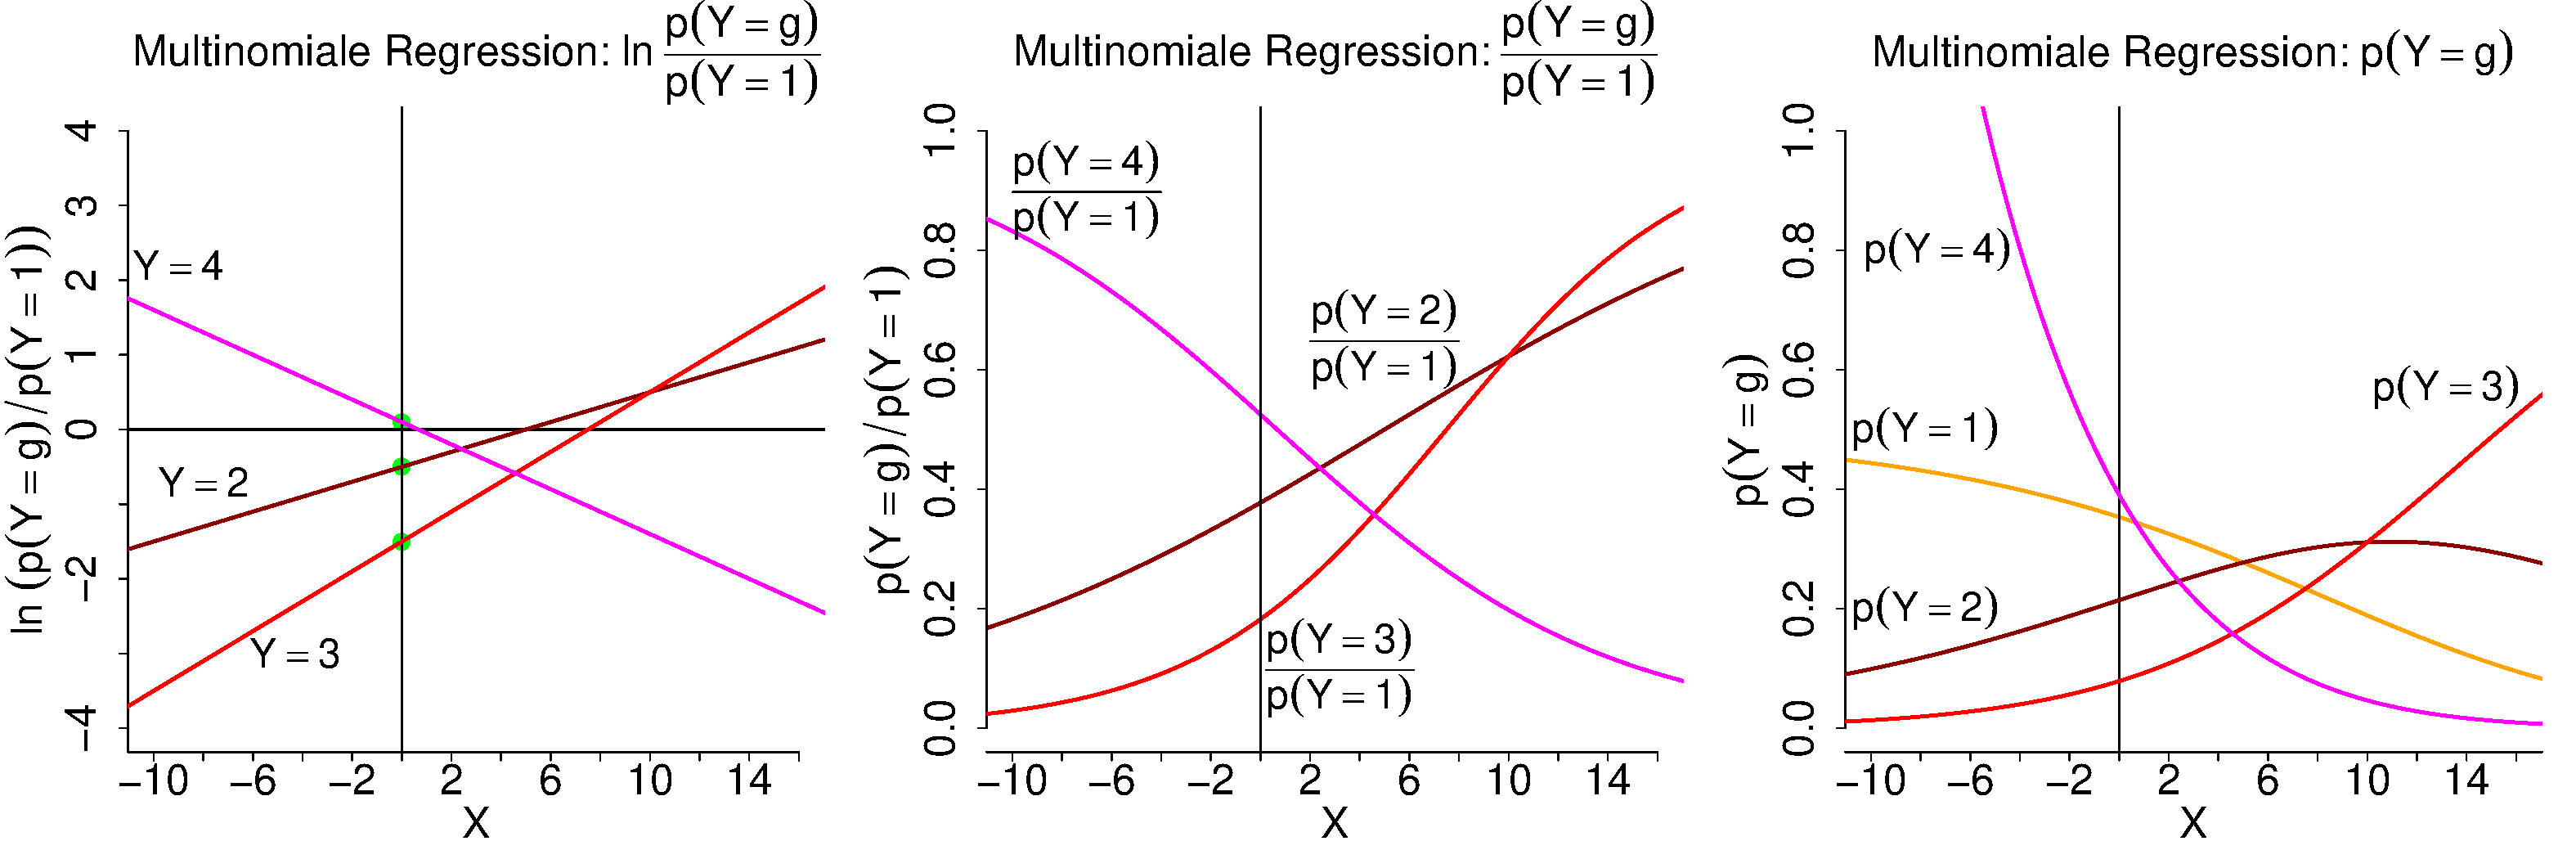
\includegraphics[width=12.5cm]{regrMultNom}
\vspace*{-0.5em}
\caption{Multinomiale Regression mit einem Prädiktor und $4$ Kategorien der AV $Y$: Linearität der 3 baseline category Logits mit unterschiedlichen Steigungen; logistische Funktionen für die Chance, verglichen mit der baseline Kategorie eine Kategorie $g$ zu erhalten; zugehörige Funktionen für die Wahrscheinlichkeit einer Kategorie $g$ von $Y$.}
\label{fig:regrMultNom}
\end{figure}

%%%%%%%%%%%%%%%%%%%%%%%%%%%%%%%%%%%%%%%%%%%%%%%%%%%%%%%%%%%%%%%%%%
%%%%%%%%%%%%%%%%%%%%%%%%%%%%%%%%%%%%%%%%%%%%%%%%%%%%%%%%%%%%%%%%%%
\subsection{Modellanpassung}
%%%%%%%%%%%%%%%%%%%%%%%%%%%%%%%%%%%%%%%%%%%%%%%%%%%%%%%%%%%%%%%%%%
%%%%%%%%%%%%%%%%%%%%%%%%%%%%%%%%%%%%%%%%%%%%%%%%%%%%%%%%%%%%%%%%%%

Als Beispiel sollen die Daten der ordinalen Regression in Abschn.\ \ref{sec:regrOrdFit} herangezogen werden, wobei als AV nun der dort bereits erstellte ungeordnete Faktor dient. Die Anpassung des Modells erfolgt wieder mit\index[func]{vglm()@\lstinline{vglm()}} \lstinline!vglm()! aus dem Paket\index[pack]{VGAM@\lstinline{VGAM}} \lstinline!VGAM!. Dafür ist das Argument \lstinline!family! auf \lstinline!multinomial(refLevel=1)! zu setzen, womit gleichzeitig die Referenzkategorie \lstinline!refLevel! auf die erste Stufe von $Y$ festgelegt werden kann. Wie in der logistischen Regression sind die Schätzungen $b_{j_{g}}$ zu exponenzieren, um die geschätzten odds ratios zu erhalten: $\euler^{b_{j_{g}}}$ gibt bezogen auf die Referenzkategorie an, um welchen Faktor die vorhergesagte Chance wächst, Kategorie $g$ zu erhalten, wenn sich $X_{j}$ um eine Einheit erhöht (Abschn.\ \ref{sec:glmFit}).
\begin{lstlisting}
> library(VGAM)                               # für vglm()
> vglmFitMN <- vglm(Ycateg ~ X1 + X2, family=multinomial(refLevel=1),
+                   data=dfOrd)

> exp(coef(vglmFitMN))                        # odds ratios
(Intercept):1 (Intercept):2 (Intercept):3          X1:1          X1:2
 5.812237e-02  1.579953e-11  8.460664e-20  1.019506e+00  1.162001e+00
         X1:3          X2:1          X2:2          X2:3
 1.316564e+00  9.854338e-01  9.636944e-01  8.647246e-01
\end{lstlisting}

%%%%%%%%%%%%%%%%%%%%%%%%%%%%%%%%%%%%%%%%%%%%%%%%%%%%%%%%%%%%%%%%%%
%%%%%%%%%%%%%%%%%%%%%%%%%%%%%%%%%%%%%%%%%%%%%%%%%%%%%%%%%%%%%%%%%%
\subsection{Anpassungsgüte}
%%%%%%%%%%%%%%%%%%%%%%%%%%%%%%%%%%%%%%%%%%%%%%%%%%%%%%%%%%%%%%%%%%
%%%%%%%%%%%%%%%%%%%%%%%%%%%%%%%%%%%%%%%%%%%%%%%%%%%%%%%%%%%%%%%%%%

Wie in der logistischen Regression dienen verschiedene Maße als Anhaltspunkte zur Anpassungsgüte des Modells (Abschn.\ \ref{sec:regrLogRsq}). Dazu zählt die Devianz ebenso wie das Informationskriterium AIC sowie die pseudo-$R^{2}$ Kennwerte.
\begin{lstlisting}
> deviance(vglmFitMN)           # Devianz
[1] 237.148

> AIC(vglmFitMN)                # Informationskriterium AIC
[1] 255.148

> library(DescTools)            # für PseudoR2()
> PseudoR2(vglmFitMN, which="Nagelkerke")
Nagelkerke 
0.3524506 
\end{lstlisting}

Für potentiell auftretende Probleme bei der Modellanpassung s.\ Abschn.\ \ref{sec:glmConvergence}.

%%%%%%%%%%%%%%%%%%%%%%%%%%%%%%%%%%%%%%%%%%%%%%%%%%%%%%%%%%%%%%%%%%
%%%%%%%%%%%%%%%%%%%%%%%%%%%%%%%%%%%%%%%%%%%%%%%%%%%%%%%%%%%%%%%%%%
\subsection{Signifikanztests für Parameter und Modell}
%%%%%%%%%%%%%%%%%%%%%%%%%%%%%%%%%%%%%%%%%%%%%%%%%%%%%%%%%%%%%%%%%%
%%%%%%%%%%%%%%%%%%%%%%%%%%%%%%%%%%%%%%%%%%%%%%%%%%%%%%%%%%%%%%%%%%

Mit \lstinline!summary(<<vglm-Modell>>)! werden neben den Parameterschätzungen $b$ auch ihre geschätzten Streuungen $\hat{\sigma}_{b}$ sowie die zugehörigen $z$-Werte $\frac{b}{\hat{\sigma}_{b}}$ berechnet. Mit der Annahme, dass $z$ unter der Nullhypothese asymptotisch standardnormalverteilt ist, stehen die zweiseitigen $p$-Werte in der Spalte \lstinline!Pr(>|z|)!. Die genannten Werte lassen sich mit \lstinline!coef(summary(<<vglm-Modell>>))! extrahieren. Profile-Likelihood Konfidenzintervalle erzeugt\index[func]{confint()@\lstinline{confint()}} \lstinline!confint(<<vglm-Modell>>, method="profile")!.
\begin{lstlisting}
> sumMN   <- summary(vglmFitMN)
> (coefMN <- coef(sumMN))
                  Estimate  Std. Error    z value     Pr(>|z|)
(Intercept):1  -2.84520460  8.86963583 -0.3207803 7.483769e-01
(Intercept):2 -24.87104089  9.67909358 -2.5695630 1.018269e-02
(Intercept):3 -43.91627419 11.63358071 -3.7749576 1.600349e-04
X1:1            0.01931815  0.05232332  0.3692072 7.119733e-01
X1:2            0.15014353  0.05662132  2.6517138 8.008439e-03
X1:3            0.27502499  0.06780602  4.0560557 4.990836e-05
X2:1           -0.01467332  0.03810166 -0.3851098 7.001561e-01
X2:2           -0.03698110  0.04095569 -0.9029539 3.665504e-01
X2:3           -0.14534420  0.04957956 -2.9315347 3.372917e-03

> confint(vglmFitMN, method="profile")
                     2.5 %       97.5 %
(Intercept):1 -20.56920320  14.58795777
(Intercept):2 -44.96340309  -6.70036945
(Intercept):3 -68.62626636 -22.65578477
X1:1           -0.08343008   0.12414067
X1:2            0.04419509   0.26805364
X1:3            0.15163779   0.41929882
X2:1           -0.09083943   0.06011880
X2:2           -0.11967388   0.04239173
X2:3           -0.24960539  -0.05352069
\end{lstlisting}

Da jeder Prädiktor mit mehreren Parametern $\beta_{j_{g}}$ assoziiert ist, müssen Prädiktoren selbst über Modellvergleiche auf Signifikanz getestet werden (Abschn.\ \ref{sec:regrLogTest}). Dazu dienen Likelihood-Quotienten-Tests, die auf der asymptotisch $\chi^{2}$-verteilten Devianz-Differenz zweier nested Modelle mit demselben Kriterium beruhen: Der Prädiktorensatz des eingeschränkten Modells \lstinline!<<fitR>>! ist dabei vollständig im Prädiktorensatz des umfassenderen Modells \lstinline!<<fitU>>! enthalten, das zusätzlich noch weitere Prädiktoren berücksichtigt. Der Test erfolgt dann mit\index[func]{anova()@\lstinline{anova()}} \lstinline!anova(<<fitR>>, <<fitU>>, type="I")!. Der $p$-Wert steht in der Ausgabe in der Spalte \lstinline!Pr(>Chi)!.
\begin{lstlisting}
# eingeschränktes Modell ohne Prädiktor X2
> vglmFitR <- vglm(Ycateg ~ X1, family=multinomial(refLevel=1),
+                  data=dfOrd)

> anova(vglmFitR, vglmFitMN, type="I")        # Modellvergleich
Analysis of Deviance Table
Model 1: Ycateg ~ X1
Model 2: Ycateg ~ X1 + X2
  Resid. Df Resid. Dev Df Deviance Pr(>Chi)   
1       294     249.00                        
2       291     237.15  3   11.852 0.007906 **
\end{lstlisting}

%%%%%%%%%%%%%%%%%%%%%%%%%%%%%%%%%%%%%%%%%%%%%%%%%%%%%%%%%%%%%%%%%%
%%%%%%%%%%%%%%%%%%%%%%%%%%%%%%%%%%%%%%%%%%%%%%%%%%%%%%%%%%%%%%%%%%
\subsection{Vorhersage, Klassifikation und Anwendung auf neue Daten}
%%%%%%%%%%%%%%%%%%%%%%%%%%%%%%%%%%%%%%%%%%%%%%%%%%%%%%%%%%%%%%%%%%
%%%%%%%%%%%%%%%%%%%%%%%%%%%%%%%%%%%%%%%%%%%%%%%%%%%%%%%%%%%%%%%%%%

Die vorhergesagten Kategorienwahrscheinlichkeiten $\hat{P}(Y = g)$ erhält man wie in der logistischen Regression mit\index[func]{predict()@\lstinline{predict()}} \lstinline!predict(<<vglm-Modell>>, type="response")!. Die ausgegebene Matrix enthält für jede Beobachtung (Zeilen) die vorhergesagte Wahrscheinlichkeit für jede Kategorie (Spalten). Mit der gewählten Herangehensweise ist die mittlere vorhergesagte Wahrscheinlichkeit für jede Kategorie gleich der empirischen relativen Häufigkeit der Kategorie.\footnote{Dies ist der Fall, wenn die kanonische Link-Funktion und Maximum-Likelihood-Schätzungen der Parameter gewählt werden und das Modell die absoluten Terme $\beta_{0_{g}}$ besitzt.}
\begin{lstlisting}
> PhatCateg <- predict(vglmFitMN, type="response")
> head(PhatCateg, n=3)
         --         -         +         ++
1 0.1946834 0.2255730 0.2982816 0.28146203
2 0.3219964 0.3219154 0.2675170 0.08857120
3 0.4473732 0.3769135 0.1596527 0.01606071

# mittlere vorhergesagte Kategorien-Wahrscheinlichkeiten
> colMeans(PhatCateg)
  --    -    +   ++
0.25 0.25 0.25 0.25

# empirische relative Kategorien-Häufigkeiten
> proportions(table(dfOrd$Ycateg))
  --    -    +   ++
0.25 0.25 0.25 0.25
\end{lstlisting}

Die vorhergesagten Kategorien selbst lassen sich aus den vorhergesagten Kategorienwahrscheinlichkeiten bestimmen, indem pro Beobachtung die Kategorie mit der maximalen vorhergesagten Wahrscheinlichkeit herangezogen wird. Das zeilenweise Maximum einer Matrix gibt \lstinline!max.col(<<Matrix>>)! aus.
\begin{lstlisting}
> categHat <- levels(dfOrd$Ycateg)[max.col(PhatCateg)]
> head(categHat)
[1] "+"  "--"  "--"  "+"  "--" "+"
\end{lstlisting}

Die Kontingenztafel tatsächlicher und vorhergesagter Kategorien eignet sich als Grundlage für die Berechnung von Übereinstimmungsmaßen wie der Rate der korrekten Klassifikation. Hier ist darauf zu achten, dass die Kategorien identisch geordnet sind.
\begin{lstlisting}
> facHat <- factor(categHat, levels=levels(dfOrd$Ycateg))
> cTab   <- table(dfOrd$Ycateg, facHat, dnn=c("Ycateg", "facHat"))
> addmargins(cTab)                      # Randsummen hinzufügen
            facHat
Ycateg  --   -   +  ++ Sum
   --    9   5   8   3  25
   -    11   5   5   4  25
   +     5   5   8   7  25
   ++    1   2   8  14  25
   Sum  26  17  29  28 100

> (CCR <- sum(diag(cTab)) / sum(cTab))  # Rate der korrekten Klass.
[1] 0.36
\end{lstlisting}

An das Argument \lstinline!newdata! von \lstinline!predict()! kann zusätzlich ein Datensatz übergeben werden, der neue Daten für Variablen mit denselben Namen, und bei Faktoren zusätzlich denselben Stufen wie jene der ursprünglichen Prädiktoren enthält. Als Ergebnis erhält man die vorhergesagten Kategorienwahrscheinlichkeiten für die neuen Prädiktorwerte (Abschn.\ \ref{sec:predict}).
\begin{lstlisting}
> Nnew  <- 3                            # Anzahl neuer Daten
> dfNew <- data.frame(X1=rnorm(Nnew, 175, 7),         # neue Daten
+                     X2=rnorm(Nnew,  30, 8))

> predict(vglmFitMN, newdata=dfNew, type="response")  # Vorhersage
          --          -         +         ++
1 0.05150391 0.06762012 0.2943623 0.58651367
2 0.45228458 0.39748171 0.1311896 0.01904412
3 0.15948745 0.18932511 0.3110646 0.34012280
\end{lstlisting}

%%%%%%%%%%%%%%%%%%%%%%%%%%%%%%%%%%%%%%%%%%%%%%%%%%%%%%%%%%%%%%%%%%
%%%%%%%%%%%%%%%%%%%%%%%%%%%%%%%%%%%%%%%%%%%%%%%%%%%%%%%%%%%%%%%%%%
\section{Regression für Zähldaten}
\label{sec:regrCount}
%%%%%%%%%%%%%%%%%%%%%%%%%%%%%%%%%%%%%%%%%%%%%%%%%%%%%%%%%%%%%%%%%%
%%%%%%%%%%%%%%%%%%%%%%%%%%%%%%%%%%%%%%%%%%%%%%%%%%%%%%%%%%%%%%%%%%

Das GLM bietet verschiedene Möglichkeiten zur Modellierung einer Variable $Y$, die nur ganzzahlige nichtnegative Werte annehmen kann und keine obere Schranke aufweist, wie es für Zähldaten charakteristisch ist. Die von $Y$ gezählten Ereignisse sollen dabei unabhängig voneinander eintreten. Handelt es sich bei den Prädiktoren $X_{j}$ um kontinuierliche Variablen, spricht man von Regressionsmodellen, bei der Modellierung einer festen Gesamtzahl von Ereignissen durch Gruppierungsfaktoren meist von log-linearen Modellen (Abschn.\ \ref{sec:loglin}).

%%%%%%%%%%%%%%%%%%%%%%%%%%%%%%%%%%%%%%%%%%%%%%%%%%%%%%%%%%%%%%%%%%
%%%%%%%%%%%%%%%%%%%%%%%%%%%%%%%%%%%%%%%%%%%%%%%%%%%%%%%%%%%%%%%%%%
\subsection{Poisson-Regression}
\label{sec:regrPoisson}
%%%%%%%%%%%%%%%%%%%%%%%%%%%%%%%%%%%%%%%%%%%%%%%%%%%%%%%%%%%%%%%%%%
%%%%%%%%%%%%%%%%%%%%%%%%%%%%%%%%%%%%%%%%%%%%%%%%%%%%%%%%%%%%%%%%%%

\index{Regression!Poisson-Regression}
\index{Poisson-Regression|see{Regression}}
Bei der Poisson-Regression wird als bedingte Verteilung von $Y$ eine Poisson-Verteilung $P(Y=y) = \frac{\mu^{y} \euler^{-\mu}}{y!}$ angenommen, mit dem Erwartungswert $\mu = E(Y)$. Die kanonische Link-Funktion ist der natürliche Logarithmus, das lineare Modell ist also $\ln \mu = \beta_{0} + \beta_{1} X_{1} + \dots + \beta_{p} X_{p} = \bm{X} \bm{\beta}$. Die bedingten Verteilungen von $Y$ sind dann bereits vollständig festgelegt, da ihre Varianz ebenfalls gleich $\mu$ ist. Der Erwartungswert ist als $\mu = \euler^{\bm{X} \bm{\beta}} = \euler^{\beta_{0}} \, \euler^{\beta_{1} X_{1}} \cdot \ldots \cdot \euler^{\beta_{p} X_{p}}$ identifizierbar. Einem exponenzierten Parameter $\euler^{\beta_{j}}$ kommt deshalb die Bedeutung des multiplikativen Faktors zu, mit dem $\mu$ wächst, wenn sich der Prädiktor $X_{j}$ um eine Einheit vergrößert.\footnote{Für einen Prädiktor $X$: $\mu_{X+1} = \euler^{\beta_{0} + \beta_{1} (X + 1)} = \euler^{\beta_{0}} \, \euler^{\beta_{1} (X + 1)} = \euler^{\beta_{0}} \, \euler^{\beta_{1} X} \, \euler^{\beta_{1}} = \euler^{\beta_{1}} \, \euler^{\beta_{0} + \beta_{1} X} = \euler^{\beta_{1}} \, \mu_{X}$.}

Die Anpassung einer Poisson-Regression geschieht wie in der logistischen Regression mit \lstinline!glm()!\index[func]{glm()@\lstinline{glm()}}, wobei das Argument \lstinline!family! auf \lstinline!poisson(link="log")! zu setzen ist (Abschn.\ \ref{sec:glmFit}).\footnote{Bei der Verwendung von\index[func]{vglm()@\lstinline{vglm()}} \lstinline!vglm()! aus dem Paket\index[pack]{VGAM@\lstinline{VGAM}} \lstinline!VGAM! ist das Argument \lstinline!family! auf \lstinline!poissonff! zu setzen.} Die Daten der vorherzusagenden Variable müssen aus ganzzahligen Werten $\geq 0$ bestehen.

Für ein Beispiel sollen zunächst Zähldaten simuliert werden, die mit zwei Prädiktoren korrelieren. Dazu wird die\index[func]{rmvnorm()@\lstinline{rmvnorm()}} \lstinline!rmvnorm()! Funktion des \lstinline!mvtnorm!\index[pack]{mvtnorm@\lstinline{mvtnorm}} Pakets verwendet, die Zufallsvektoren einer multinormalverteilten Variable simuliert. Die Verwendung von \lstinline!rmvnorm()! gleicht der von \lstinline!rnorm()!, lediglich muss hier das theoretische Zentroid $\bm{\mu}$ für das Argument \lstinline!mean! und die theoretische Kovarianzmatrix $\bm{\Sigma}$ für \lstinline!sigma! angegeben werden. Die Daten einer der erzeugten Variablen werden zusätzlich gerundet und ihre negativen Werte auf Null gesetzt, damit sie als Zählvariable dienen kann.
\begin{lstlisting}
> library(mvtnorm)                              # für rmvnorm()
> N     <- 200
> sigma <- matrix(c(4,2,-3, 2,16,-1, -3,-1,8), byrow=TRUE, ncol=3)
> mu    <- c(-3, 2, 4)                          # Erwartungswerte
> XY    <- rmvnorm(N, mean=mu, sigma=sigma)     # Zufallsdaten
> Y     <- round(XY[ , 3] - 1.5)                # runde Zähldaten
> Y[Y < 0] <- 0                                 # negative Werte -> 0
> dfCount <- data.frame(X1=XY[ , 1], X2=XY[ , 2], Y)    # Datensatz

# Poisson-Regression
> glmFitP <- glm(Y ~ X1 + X2, family=poisson(link="log"), data=dfCount)
\end{lstlisting}

Wie in der logistischen Regression erhält man die Parameterschätzungen $b_{j}$ mit \lstinline!coef()! und die Konfidenzintervalle für die Parameter $\beta_{j}$ mit \lstinline!confint()! (Abschn.\ \ref{sec:glmFit}, Fußnote \ref{ftn:ciDefault}). Die geschätzten Änderungsfaktoren für $E(Y)$ ergeben sich durch Exponenzieren als $\euler^{b_{j}}$.
\begin{lstlisting}
> exp(coef(glmFitP))                  # Änderungsfaktoren
(Intercept)          X1          X2
  1.1555238   0.7692037   1.0205773

> exp(confint(glmFitP))               # zugehörige Konfidenzintervalle
                2.5 %    97.5 %
(Intercept) 0.9479450 1.3993779
X1          0.7380968 0.8015816
X2          0.9992731 1.0424328
\end{lstlisting}

Wald-Tests der Parameter und Informationen zur Modellpassung insgesamt liefert \lstinline!summary()! (Abschn.\ \ref{sec:regrLogRsq}, \ref{sec:regrLogTest}).
\begin{lstlisting}
> summary(glmFitP)   # Parametertests + Modellpassung, gekürzte Ausgabe
Deviance Residuals:
    Min       1Q   Median       3Q      Max
-3.1695  -1.4608  -0.2707   0.7173   3.4757

Coefficients:
            Estimate Std. Error z value Pr(>|z|)
(Intercept)  0.14455    0.09935   1.455    0.146
X1          -0.26240    0.02105 -12.466   <2e-16 ***
X2           0.02037    0.01079   1.888    0.059 .

(Dispersion parameter for poisson family taken to be 1)

    Null deviance: 536.93  on 199  degrees of freedom
Residual deviance: 374.78  on 197  degrees of freedom
AIC: 825.22

Number of Fisher Scoring iterations: 5
\end{lstlisting}

Wie in der logistischen Regression erhält man die vorhergesagten Häufigkeiten mit \lstinline!predict(<<glm-Modell>>, type="response")! (Abschn.\ \ref{sec:logisticPred}). Über das Argument \lstinline!newdata! lässt sich das angepasste Modell dabei auch auf neue Werte für dieselben Prädiktoren anwenden, um Vorhersagen zu gewinnen.

%%%%%%%%%%%%%%%%%%%%%%%%%%%%%%%%%%%%%%%%%%%%%%%%%%%%%%%%%%%%%%%%%%
%%%%%%%%%%%%%%%%%%%%%%%%%%%%%%%%%%%%%%%%%%%%%%%%%%%%%%%%%%%%%%%%%%
\subsection{Ereignisraten analysieren}
\label{sec:poissonRate}
%%%%%%%%%%%%%%%%%%%%%%%%%%%%%%%%%%%%%%%%%%%%%%%%%%%%%%%%%%%%%%%%%%
%%%%%%%%%%%%%%%%%%%%%%%%%%%%%%%%%%%%%%%%%%%%%%%%%%%%%%%%%%%%%%%%%%

Die Poisson-Regression erlaubt es auch, Ereignisraten zu analysieren. Die absoluten Häufigkeiten $Y$ sind dann auf eine bestimmte Referenzgröße $t$ bezogen, die die Menge der potentiell beobachtbaren Ereignisse bestimmt. Bei $t$ kann es sich etwa um die Länge eines Zeitintervalls handeln, in dem Ereignisse gezählt werden. In einer anderen Situation kann $t$ die Größe einer Fläche sein, auf der die Anzahl von Elementen mit einer bestimmten Eigenschaft zu zählen sind, die jeweils einem Ereignis entsprechen. $t$ wird als \emph{exposure} bezeichnet und ist echt positiv.

Bezeichnet $t$ die Zeitdauer, nimmt man an, dass der Abstand zwischen zwei aufeinander folgenden Ereignissen unabhängig von $t$ exponentialverteilt mit Erwartungwert $\frac{1}{\lambda}$ ist. Dann folgt $E(Y) = \lambda \, t$ mit der Konstante $\lambda$ als echt positiver Grundrate, mit der ein Ereignis pro Zeiteinheit auftritt.

Ist in einer Untersuchung die zu den beobachteten Häufigkeiten $Y$ gehörende exposure $t$ variabel, stellt die Grundrate $\lambda = \frac{\mu}{t}$ die zu modellierende Variable dar. Mit dem Logarithmus als Link-Funktion folgt $\bm{X} \bm{\beta} = \ln \lambda = \ln \frac{\mu}{t} = \ln \mu - \ln t$, als lineares Vorhersagemodell ergibt sich $\ln \mu = \bm{X} \bm{\beta} + \ln t$. Im linearen Prädiktor $1 \ln t + \beta_{0} + \beta_{1} X_{1} + \dots + \beta_{p} X_{p}$ ist $1 \ln t$ eine additive Konstante wie $\beta_{0}$ -- allerdings mit dem Unterschied, dass $t$ durch die Daten festgelegt ist und das zugehörige auf $1$ fixierte Regressionsgewicht nicht geschätzt werden muss. $\ln t$ wird als \emph{offset} bezeichnet. Die Grundrate $\lambda$ ist identifizierbar als $\lambda = \euler^{\bm{X} \bm{\beta} + \ln t} = t \, \euler^{\bm{X} \bm{\beta}}$.

In der Anpassung der Poisson-Regression für Ereignisraten mit \lstinline!glm()! ist das Argument \lstinline!offset=log(<<t>>)! zu verwenden. Dabei ist \lstinline!<<t>>! ein Vektor mit den Werten der exposure.
\begin{lstlisting}
# simulierte Zähldaten, hier ohne Zusammenhang Prädiktor - Zielgröße
> Nt   <- 100                               # Beobachtungsobjekte
> Ti   <- sample(20:40, Nt, replace=TRUE)   # exposure
> Xt   <- rnorm(Nt, 100, 15)                # Prädiktor
> Yt   <- rbinom(Nt, size=Ti, prob=0.5)     # beobachtete Häufigkeiten
> fitT <- glm(Yt ~ Xt, family=poisson(link="log"), offset=log(Ti))
> summary(fitT)                             # ...
\end{lstlisting}

%%%%%%%%%%%%%%%%%%%%%%%%%%%%%%%%%%%%%%%%%%%%%%%%%%%%%%%%%%%%%%%%%%
%%%%%%%%%%%%%%%%%%%%%%%%%%%%%%%%%%%%%%%%%%%%%%%%%%%%%%%%%%%%%%%%%%
\subsection{Adjustierte Poisson-Regression und negative Binomial-Regression}
%%%%%%%%%%%%%%%%%%%%%%%%%%%%%%%%%%%%%%%%%%%%%%%%%%%%%%%%%%%%%%%%%%
%%%%%%%%%%%%%%%%%%%%%%%%%%%%%%%%%%%%%%%%%%%%%%%%%%%%%%%%%%%%%%%%%%

\index{Regression!negative Binomial-Regression}
Oft streuen empirische Residuen deutlich stärker, als dies bei bedingter Poisson-Verteilung von $Y$ zu erwarten wäre, bei der die Streuung gleich dem bedingten Erwartungswert ist (\emph{overdispersion}). Ein Hinweis auf overdispersion ist ein Verhältnis von Residual-Devianz zu Residual-Freiheitsgraden, das deutlich größer als $1$ ist. Bei overdispersion kann ein Poisson-ähnliches Modell verwendet werden, das einen zusätzlichen, aus den Daten zu schätzenden Streuungsparameter $\phi$ besitzt, mit dem für die bedingte Varianz $\sigma^{2} = \phi \mu$ gilt. Hierfür ist das Argument \lstinline!family! von \lstinline!glm()! auf \lstinline!quasipoisson(link="log")! zu setzen. Dies führt zu identischen Parameterschätzungen $b$, jedoch zu anderen geschätzten Streuungen $\hat{\sigma}_{b}$ und damit zu anderen Ergebnissen der inferenzstatistischen Tests. Abschnitt \ref{sec:glmOtherLink} erläutert mögliche Ursachen von overdispersion und Konsequenzen der Verwendung von quasi-Familien.
\begin{lstlisting}
> glmFitQP <- glm(Y ~ X1 + X2, family=quasipoisson(link="log"),
+                 data=dfCount)

> summary(glmFitQP)                  # gekürzte Ausgabe ...
Deviance Residuals:
    Min       1Q   Median       3Q      Max
-3.1695  -1.4608  -0.2707   0.7173   3.4757

Coefficients:
            Estimate Std. Error t value Pr(>|t|)
(Intercept)  0.14455    0.12943   1.117    0.265
X1          -0.26240    0.02742  -9.569   <2e-16 ***
X2           0.02037    0.01405   1.450    0.149

(Dispersion parameter for quasipoisson family taken to be 1.697012)

    Null deviance: 536.93  on 199  degrees of freedom
Residual deviance: 374.78  on 197  degrees of freedom
AIC: NA
\end{lstlisting}

Für eine adjustierte Poisson-Regression kann alternativ auch ein separater robuster Streuungsschätzer verwendet werden, wie ihn etwa das Paket\index[pack]{sandwich@\lstinline{sandwich}} \lstinline!sandwich! mit\index[func]{vcovHC()@\lstinline{vcovHC()}} \lstinline!vcovHC()! bereitstellt (Abschn.\ \ref{sec:lmRob}). Wald-Tests der Parameter lassen sich dann mit\index[func]{coeftest()@\lstinline{coeftest()}} \lstinline!coeftest(<<glm-Modell>>, vcov=<<Schätzer>>)! aus dem Paket \index[pack]{lmtest@\lstinline{lmtest}} \lstinline!lmtest! durchführen, wobei für das Argument \lstinline!vcov! das Ergebnis von \lstinline!vcovHC()! anzugeben ist.
\begin{lstlisting}
> library(sandwich)                           # für vcovHC()
> hcSE <- vcovHC(glmFitP, type="HC0")         # robuste SE-Schätzung
> library(lmtest)                             # für coeftest()
> coeftest(glmFitP, vcov=hcSE)                # Parametertests
z test of coefficients:

             Estimate Std. Error  z value Pr(>|z|)
(Intercept)  0.144554   0.135709  1.0652   0.2868
X1          -0.262399   0.028753 -9.1259   <2e-16 ***
X2           0.020368   0.013097  1.5552   0.1199
\end{lstlisting}

Eine weitere Alternative ist die Regression mit der Annahme, dass die bedingte Verteilung von $Y$ eine negative Binomialverteilung ist, die einen eigenen Dispersionsparameter $\theta$ besitzt. Sie verallgemeinert die Poisson-Verteilung mit demselben Erwartungswert $\mu$, ihre Varianz ist jedoch mit $\mu + \frac{\mu^{2}}{\theta} = \mu (1 + \frac{\mu}{\theta})$ um den Faktor $1 + \frac{\mu}{\theta}$ größer. Die negative Binomial-Regression lässt sich mit\index[func]{glm.nb()@\lstinline{glm.nb()}} \lstinline!glm.nb()! aus dem Paket\index[pack]{MASS@\lstinline{MASS}} \lstinline!MASS! anpassen.\footnote{Bei der Verwendung von\index[func]{vglm()@\lstinline{vglm()}} \lstinline!vglm()! aus dem Paket\index[pack]{VGAM@\lstinline{VGAM}} \lstinline!VGAM! ist das Argument \lstinline!family! auf \lstinline!negbinomial! zu setzen.}
\begin{lstlisting}
> library(MASS)                               # für glm.nb()
> glmFitNB <- glm.nb(Y ~ X1 + X2, data=dfCount)
> summary(glmFitNB)                           # gekürzte Ausgabe ...
Deviance Residuals:
    Min       1Q   Median       3Q      Max
-2.6146  -1.2540  -0.2149   0.5074   2.7341

Coefficients:
              Estimate Std. Error z value Pr(>|z|)
(Intercept)  0.003337   0.130007   0.026   0.9795
X1          -0.302121   0.029972 -10.080   <2e-16 ***
X2           0.025419   0.014649   1.735   0.0827 .

(Dispersion parameter for Negative Binomial(3.85) family taken to be 1)

    Null deviance: 353.34  on 199  degrees of freedom
Residual deviance: 250.31  on 197  degrees of freedom
AIC: 801.11

Number of Fisher Scoring iterations: 1

              Theta:  3.85
          Std. Err.:  1.12
 2 x log-likelihood:  -793.113
\end{lstlisting}

Das Ergebnis nennt neben den bekannten Kennwerten unter \lstinline!Theta! eine Schätzung für den Dispersionsparameter $\theta$. Das von \lstinline!glm.nb()! erzeugte Objekt kann an die Funktion\index[func]{odTest()@\lstinline{odTest()}} \lstinline!odTest()! aus dem Paket\index[pack]{pscl@\lstinline{pscl}} \lstinline!pscl! \cite{Zeileis2008} übergeben werden. Sie führt dann einen Test auf overdispersion durch, der auf dem Vergleich der Anpassungsgüte von Poisson- und negativem Binomial-Modell beruht.
\begin{lstlisting}
> library(pscl)                               # für odTest()
> odTest(glmFitNB)                            # overdispersion-Test
Likelihood ratio test of H0: Poisson, as restricted NB model:
n.b., the distribution of the test-statistic under H0 is non-standard
e.g., see help(odTest) for details/references

Critical value of test statistic at the alpha= 0.05 level: 2.7055
Chi-Square Test Statistic = 26.1033 p-value = 1.618e-07
\end{lstlisting}

%%%%%%%%%%%%%%%%%%%%%%%%%%%%%%%%%%%%%%%%%%%%%%%%%%%%%%%%%%%%%%%%%%
%%%%%%%%%%%%%%%%%%%%%%%%%%%%%%%%%%%%%%%%%%%%%%%%%%%%%%%%%%%%%%%%%%
\subsection{Zero-inflated Poisson-Regression}
%%%%%%%%%%%%%%%%%%%%%%%%%%%%%%%%%%%%%%%%%%%%%%%%%%%%%%%%%%%%%%%%%%
%%%%%%%%%%%%%%%%%%%%%%%%%%%%%%%%%%%%%%%%%%%%%%%%%%%%%%%%%%%%%%%%%%

\index{Regression!zero-inflated Modelle}
Eine mögliche Quelle für starke Streuungen von Zähldaten sind gehäuft auftretende Nullen. Sie können das Ergebnis eines zweistufigen Prozesses sein, mit dem die Daten zustande kommen. Wird etwa erfasst, wie häufig Personen im Beruf befördert werden oder ihren Arbeitsplatz wechseln, ist zunächst relevant, ob sie überhaupt jemals eine Arbeitsstelle erhalten haben. Diese Eigenschaft wird vermutlich durch qualitativ andere Prozesse bestimmt als jene, die bei tatsächlich Erwerbstätigen die Anzahl der unterschiedlichen Positionen beeinflussen. Die Daten können damit als Ergebnis einer Mischung von zwei Verteilungen verstanden werden: Zum einen kommen Nullen durch Personen zustande, die ein notwendiges Kriterium für einen auch zu echt positiven Häufigkeiten führenden Prozess nicht erfüllen. Zum anderen verursachen Personen, die ein solches Kriterium erfüllen, ihrerseits Nullen sowie zusätzlich echt positive Häufigkeiten. Für die Daten dieser zweiten Gruppe von Personen kann nun wieder angenommen werden, dass sie sich durch eine Poisson- oder negative Binomialverteilung beschreiben lassen.

In der geschilderten Situation kommen \emph{zero-inflated} Modelle in Betracht. Sie sorgen durch die Annahme einer Mischverteilung letztlich dafür, dass im Modell eine deutlich höhere Auftretenswahrscheinlichkeit von Nullen möglich ist, als es zur Verteilung der echt positiven Häufigkeiten passt.

Die zero-inflated Poisson-Regression eignet sich für Situationen, in denen keine starke overdispersion zu vermuten ist und kann mit\index[func]{zeroinfl()@\lstinline{zeroinfl()}} \lstinline!zeroinfl()! aus dem Paket \lstinline!pscl! angepasst werden (für Details vgl.\ \lstinline!vignette("countreg")!).\footnote{Bei der Verwendung von\index[func]{vglm()@\lstinline{vglm()}} \lstinline!vglm()! aus dem Paket\index[pack]{VGAM@\lstinline{VGAM}} \lstinline!VGAM! ist das Argument \lstinline!family! auf \lstinline!zipoissonff! zu setzen.}
\begin{lstlisting}
zeroinfl(<<Modellformel>>, dist="<<Verteilung>>", offset=<<offset>>,
         data=<<Datensatz>>)
\end{lstlisting}

Die Modellformel besitzt hier die Form \lstinline!<<AV>> ~ <<UV>> | <<0-Anteil>>!. Für \lstinline!<<0-Anteil>>! ist ein Prädiktor zu nennen, der im Modell separat den Anteil der {\quotedblbase}festen{\textquotedblleft} Nullen an den Daten kontrolliert, die von jenen Personen stammen, die prinzipiell keine echt positiven Daten liefern können. Im einfachsten Fall ist dies der absolute Term \lstinline!1!, der zu einem Binomialmodell passt, das für alle Beobachtungen dieselbe Wahrscheinlichkeit vorsieht, zu dieser Gruppe zu gehören. In komplizierteren Situationen könnte die Gruppenzugehörigkeit analog zu einer separaten logistischen Regression durch einen eigenen Prädiktor vorhergesagt werden. Das Argument \lstinline!dist! ist auf \lstinline!"poisson"! zu setzen, \lstinline!data! erwartet einen Datensatz mit den Variablen aus der Modellformel. Wie bei \lstinline!glm()! existiert ein Argument \lstinline!offset! für die Analyse von Ereignisraten (Abschn.\ \ref{sec:poissonRate}).
\begin{lstlisting}
> library(pscl)                               # für zeroinfl()
> ziFitP <- zeroinfl(Y ~ X1 + X2 | 1, dist="poisson", data=dfCount)
> summary(ziFitP)                             # gekürzte Ausgabe ...
Pearson residuals:
    Min      1Q  Median      3Q     Max
-1.4805 -0.9447 -0.1574  0.6397  3.8149

Count model coefficients (poisson with log link):
            Estimate Std. Error z value Pr(>|z|)
(Intercept)  0.50809    0.13063   3.890   0.0001 ***
X1          -0.20443    0.02658  -7.692 1.45e-14 ***
X2           0.01781    0.01156   1.541   0.1233

Zero-inflation model coefficients (binomial with logit link):
            Estimate Std. Error z value Pr(>|z|)
(Intercept)  -1.4957     0.2627  -5.693 1.25e-08 ***

Number of iterations in BFGS optimization: 10
Log-likelihood: -393.1 on 4 Df
\end{lstlisting}

Separate Wald-Tests der Parameter lassen sich mit \lstinline!coeftest()! aus dem Paket\index[pack]{lmtest@\lstinline{lmtest}} \lstinline!lmtest! durchführen, Likelihood-Quotienten-Tests für nested Modelle können mit \lstinline!lrtest()! aus demselben Paket vorgenommen werden.

Die zero-inflated negative Binomial-Regression kann in Situationen mit gehäuft auftretenden Nullen und einer deutlichen overdispersion zum Einsatz kommen. Auch für sie eignet sich \lstinline!zeroinfl()!, wobei das Argument \lstinline!dist="negbin"! zu setzen ist.\footnote{Bei der Verwendung von\index[func]{vglm()@\lstinline{vglm()}} \lstinline!vglm()! aus dem Paket\index[pack]{VGAM@\lstinline{VGAM}} \lstinline!VGAM! ist das Argument \lstinline!family! auf \lstinline!zinegbinomial! zu setzen.}
\begin{lstlisting}
> ziFitNB <- zeroinfl(Y ~ X1 + X2 | 1, dist="negbin", data=dfCount)
> summary(ziFitNB)
Pearson residuals:
    Min      1Q  Median      3Q     Max
-1.4548 -0.9007 -0.1515  0.6482  3.9289

Count model coefficients (negbin with log link):
            Estimate Std. Error z value Pr(>|z|)
(Intercept)  0.36993    0.17740   2.085   0.0370 *
X1          -0.23375    0.03738  -6.254    4e-10 ***
X2           0.02111    0.01320   1.599   0.1098
Log(theta)   2.65338    0.81911   3.239   0.0012 **

Zero-inflation model coefficients (binomial with logit link):
            Estimate Std. Error z value Pr(>|z|)
(Intercept)  -1.7486     0.3924  -4.457 8.33e-06 ***

Theta = 14.2019
Number of iterations in BFGS optimization: 20
Log-likelihood:  -392 on 5 Df
\end{lstlisting}

Der\index{Vuong-Test} Vuong-Test vergleicht die Anpassungsgüte eines von \lstinline!glm()! erstellten Poisson-Modells mit jener des durch \lstinline!zeroinfl()! erstellten zero-inflated Poisson-Modells und kann mit\index[func]{vuong()@\lstinline{vuong()}} \lstinline!vuong()! aus dem Paket \lstinline!pscl! durchgeführt werden. Analog testet \lstinline!vuong()! auch ein mit \lstinline!glm.nb()! angepasstes negatives Binomial-Modell gegen das zero-inflated negative Binomial-Modell aus \lstinline!zeroinfl()!.
\begin{lstlisting}
# Poisson-Modell vs. zero-inflated Poisson-Modell
> library(pscl)                               # für vuong()
> vuong(ziFitP, glmFitP)
Vuong Non-Nested Hypothesis Test-Statistic: -0.4582521
(test-statistic is asymptotically distributed N(0,1) under the
null that the models are indistinguishible)
in this case:
model2 > model1, with p-value 0.32339

# negatives Binomial- vs. zero-inflated negatives Binomial-Modell
> vuong(ziFitNB, glmFitNB)
Vuong Non-Nested Hypothesis Test-Statistic: -1.382096
(test-statistic is asymptotically distributed N(0,1) under the
null that the models are indistinguishible)
in this case:
model2 > model1, with p-value 0.083471
\end{lstlisting}

Eine Alternative zu zero-inflated Modellen bei gehäuft auftretenden Nullen ist die\index{Regression!Hurdle-Regression} Hurdle-Regression, die von\index[func]{hurdle()@\lstinline{hurdle()}} \lstinline!hurdle()! aus dem Paket \lstinline!pscl! umgesetzt wird.

%%%%%%%%%%%%%%%%%%%%%%%%%%%%%%%%%%%%%%%%%%%%%%%%%%%%%%%%%%%%%%%%%%
%%%%%%%%%%%%%%%%%%%%%%%%%%%%%%%%%%%%%%%%%%%%%%%%%%%%%%%%%%%%%%%%%%
\subsection{Zero-truncated Poisson-Regression}
%%%%%%%%%%%%%%%%%%%%%%%%%%%%%%%%%%%%%%%%%%%%%%%%%%%%%%%%%%%%%%%%%%
%%%%%%%%%%%%%%%%%%%%%%%%%%%%%%%%%%%%%%%%%%%%%%%%%%%%%%%%%%%%%%%%%%

\index{Regression!zero-truncated Modelle}
Im Gegensatz zum Umstand gehäuft auftretender Nullen erzwingt der Aufbau mancher Untersuchungen, dass \emph{keine} Nullen beobachtet werden können. Dies ist etwa der Fall, wenn mindestens ein Ereignis vorliegen muss, damit eine Untersuchungseinheit in der Erhebung berücksichtigt wird: So ließe sich an bereits stationär aufgenommenen Patienten die Anzahl der Tage erheben, die sie im Krankenhaus verbringen, oder es könnte die Anzahl geborener Hundewelpen eines Wurfes erfasst werden. Zur Modellierung solcher Variablen kommen beschränkte (\emph{zero-truncated}) Verteilungen in Frage, die den Wert $0$ nur mit Wahrscheinlichkeit Null annehmen. Dazu zählen die zero-truncated Poisson-Verteilung -- für Situationen ohne overdispersion -- sowie die zero-truncated negative Binomialverteilung -- bei overdispersion. Um sie bei der Modellanpassung mit \lstinline!vglm()! aus dem Paket \lstinline!VGAM! zu verwenden, ist das Argument \lstinline!family! auf \lstinline!pospoisson! bzw.\ auf \lstinline!posnegbinomial! zu setzen.

%%%%%%%%%%%%%%%%%%%%%%%%%%%%%%%%%%%%%%%%%%%%%%%%%%%%%%%%%%%%%%%%%%
%%%%%%%%%%%%%%%%%%%%%%%%%%%%%%%%%%%%%%%%%%%%%%%%%%%%%%%%%%%%%%%%%%
\section{Log-lineare Modelle}
\label{sec:loglin}
%%%%%%%%%%%%%%%%%%%%%%%%%%%%%%%%%%%%%%%%%%%%%%%%%%%%%%%%%%%%%%%%%%
%%%%%%%%%%%%%%%%%%%%%%%%%%%%%%%%%%%%%%%%%%%%%%%%%%%%%%%%%%%%%%%%%%

Log-lineare Modelle analysieren den Zusammenhang mehrerer kategorialer Variablen auf Basis ihrer gemeinsamen Häufigkeitsverteilung \cite{Agresti2007}. Sie sind für Daten geeignet, die sich als mehrdimensionale Kontingenztafeln absoluter Häufigkeiten darstellen lassen und verallgemeinern damit klassische nonparametrische Tests auf Unabhängigkeit bzw.\ auf Gleichheit von bedingten Verteilungen (Abschn.\ \ref{sec:freqNonparam}, \ref{sec:assocMisc}).

%%%%%%%%%%%%%%%%%%%%%%%%%%%%%%%%%%%%%%%%%%%%%%%%%%%%%%%%%%%%%%%%%%
%%%%%%%%%%%%%%%%%%%%%%%%%%%%%%%%%%%%%%%%%%%%%%%%%%%%%%%%%%%%%%%%%%
\subsection{Modell}
\label{sec:loglinModel}
%%%%%%%%%%%%%%%%%%%%%%%%%%%%%%%%%%%%%%%%%%%%%%%%%%%%%%%%%%%%%%%%%%
%%%%%%%%%%%%%%%%%%%%%%%%%%%%%%%%%%%%%%%%%%%%%%%%%%%%%%%%%%%%%%%%%%

Aus Sicht der Datenerhebung können Kontingenztafeln absoluter Häufigkeiten aus drei Situationen entstehen. Sie sollen hier an einer $(P \times Q)$-Kontingenztafel der kategorialen Variablen $X_{1}$ und $X_{2}$ erläutert werden.
\begin{equation*}
\begin{array}{r|ccccc|l}
~        & x_{2.1} & \ldots & x_{2.q} & \ldots & x_{2.Q} & \text{Summe} \\\hline
x_{1.1}  & f_{11}  & \ldots & f_{1k}  & \ldots & f_{1q}  & f_{1+} \\
\vdots   & \vdots  & \ddots & \vdots  & \ddots & \vdots  & \vdots \\
x_{1.p}  & f_{j1}  & \ldots & f_{jk}  & \ldots & f_{jq}  & f_{p+} \\
\vdots   & \vdots  & \ddots & \vdots  & \ddots & \vdots  & \vdots \\
x_{1.P}  & f_{p1}  & \ldots & f_{pk}  & \ldots & f_{pq}  & f_{P+} \\\hline
\text{Summe} & f_{+1} & \ldots & f_{+q} & \ldots & f_{+Q} & N
\end{array}
\end{equation*}

\begin{itemize}
\item Im \emph{produkt-multinomialen} Erhebungsschema ist $X_{1}$ ein fester Faktor mit vorgegebenen Gruppenhäufigkeiten $f_{p+}$, aus deren Summe sich die feste Anzahl $N$ von Beobachtungsobjekten ergibt -- etwa in einem Experiment mit kontrollierter Zuweisung zu Versuchsbedingungen. Erhoben wird die kategoriale Variable $X_{2}$, deren Verteilung über die Gruppen $j$ i.\,S.\ der Auftretenshäufigkeiten ihrer Kategorien $f_{+q}$ zufällig ist.

\item Im \emph{multinomialen} Erhebungsschema werden mehrere kategoriale Variablen $X_{j}$ gleichzeitig an einer festen Anzahl $N$ von Beobachtungsobjekten erhoben, etwa im Rahmen einer Befragung. Die Kontingenztafel entsteht aus der Kreuzklassifikation der $X_{j}$ und gibt die Häufigkeiten an, mit der Kombinationen ihrer Kategorien auftreten. Dabei sind die $f_{p+}$ und $f_{+q}$ zufällig. In diesem Schema werden keine Einflussbeziehungen der $X_{j}$ auf eine separate Variable untersucht, sondern Zusammenhänge zwischen den $X_{j}$ selbst.

\item Im \emph{Poisson}-Erhebungsschema wird gleichzeitig mit den Ausprägungen kategorialer Einflussgrößen $X_{j}$ eine separate Variable $Y$ als Anzahl bestimmter Ereignisse erhoben. Die Kontingenztafel stellt die Anzahl der Ereignisse in den Gruppen dar, die durch die Kombination der Stufen der $X_{j}$ entstehen. Dabei ist die Gesamthäufigkeit der Ereignisse $N$ wie auch ihre Verteilung in den Gruppen der Häufigkeiten $f_{p+}$ und $f_{+q}$ zufällig. In diesem Schema nimmt man eine Poisson-Verteilung für $N$ an, womit jedes Ereignis unabhängig voneinander eintritt und als einzelne Beobachtung der Merkmalskombinationen der $X_{j}$ zählt. Bedingt auf $N$ liegt dann wieder ein multinomiales Schema vor.
\end{itemize}

Das log-lineare Modell ist ein lineares Modell für $\ln \mu_{jk}$, den logarithmierten Erwartungswert einer Zellhäufigkeit $f_{jk}$. Formuliert als Regression mit Treatment-Kontrasten hat es dieselbe Form wie das der Poisson-Regression (Abschn.\ \ref{sec:regrPoisson}). Es ist jedoch üblicher, es wie die mehrfaktorielle Varianzanalyse (Abschn.\ \ref{sec:CRFpq}) mit Effektcodierung (Abschn.\ \ref{sec:multALManova}) zu parametrisieren. Mit der Stichprobengröße $N$, der Zellwahrscheinlichkeit $p_{jk}$ und den Randwahrscheinlichkeiten $p_{p+}, p_{+q}$ analog zu den Häufigkeiten gilt dafür zunächst:
\begin{alignat*}{2}
\mu_{jk}     &= N p_{jk}           & &= N p_{p+} \, p_{+q} \, \frac{p_{jk}}{p_{p+} \, p_{+q}}\\
\ln \mu_{jk} &= \ln N + \ln p_{jk} & &= \ln N + \ln p_{p+} + \ln p_{+q} + (\ln p_{jk} - (\ln p_{p+} + \ln p_{+q}))
\end{alignat*}

Das Modell für $\ln \mu_{jk}$ hat nun für eine zweidimensionale Kontingenztafel dieselbe Form wie jenes der zweifaktoriellen Varianzanalyse mit Effektcodierung. Dabei ist $\ln N$ analog zu $\mu$, $\ln p_{p+}$ analog zu $\alpha_{j}$ (Zeileneffekt von Gruppe $j$ des Faktors $X_{1}$), $\ln p_{+q}$ analog zu $\beta_{k}$ (Spalteneffekt von Stufe $k$ des Faktors $X_{2}$) und $\ln p_{jk} - (\ln p_{p+} + \ln p_{+q})$ analog zu $(\alpha \beta)_{jk}$ (Interaktionseffekt).\footnote{Anders als in der Varianzanalyse gibt es jedoch im log-linearen Modell nur eine Beobachtung pro Zelle, die Rolle der abhängigen Variable der Varianzanalyse hat im log-linearen Modell die logarithmierte Auftretenshäufigkeit der zur Zelle gehörenden Kombination von Faktorstufen.}
\begin{align*}
\mu_{jk} &= \euler^{\mu} \, \euler^{\alpha_{j}} \, \euler^{\beta_{k}} \, \euler^{(\alpha \beta)_{jk}}\\
\ln \mu_{jk}      &= \mu + \alpha_{j} + \beta_{k} + (\alpha \beta)_{jk}\\
\end{align*}

Als Abweichung der logarithmierten Zellwahrscheinlichkeit von Additivität der logarithmierten Randwahrscheinlichkeiten drückt der Interaktionseffekt $(\alpha \beta)_{jk}$ den Zusammenhang von $X_{1}$ und $X_{2}$ aus, da bei Unabhängigkeit $p_{jk} = p_{p+} \, p_{+q}$ gilt -- logarithmiert also $\ln p_{jk} = \ln p_{p+} + \ln p_{+q}$. In zweidimensionalen Kreuztabellen sind alle beobachtbaren Zellhäufigkeiten mit dem vollständigen Modell (Zeilen-, Spalten- und Interaktionseffekt) verträglich, das deswegen als \emph{saturiert} bezeichnet wird und sich nicht testen lässt. Dagegen sind eingeschränkte Modelle wie das der Unabhängigkeit statistisch prüfbar. Für höherdimensionale Kontingenztafeln gilt dies analog, wobei kompliziertere Abhängigkeitsbeziehungen durch die Interaktionen erster und höherer Ordnung ausgedrückt werden können.

Für den Spezialfall zweidimensionaler Kreuztabellen ist das beschriebene Unabhängigkeitsmodell im multinomialen Erhebungsschema dasselbe, das vom $\chi^{2}$-Test auf Unabhängigkeit geprüft wird (Abschn.\ \ref{sec:chisqInd}). Im produkt-multinomialen Erhebungsschema ist es analog dasselbe, das der $\chi^{2}$-Test auf Gleichheit von bedingten Verteilungen testet (Abschn.\ \ref{sec:chisqEq}).

%%%%%%%%%%%%%%%%%%%%%%%%%%%%%%%%%%%%%%%%%%%%%%%%%%%%%%%%%%%%%%%%%%
%%%%%%%%%%%%%%%%%%%%%%%%%%%%%%%%%%%%%%%%%%%%%%%%%%%%%%%%%%%%%%%%%%
\subsection{Modellanpassung mit \texttt{loglm()}}
\label{sec:loglinFit}
%%%%%%%%%%%%%%%%%%%%%%%%%%%%%%%%%%%%%%%%%%%%%%%%%%%%%%%%%%%%%%%%%%
%%%%%%%%%%%%%%%%%%%%%%%%%%%%%%%%%%%%%%%%%%%%%%%%%%%%%%%%%%%%%%%%%%

Log-lineare Modelle lassen sich mit der Funktion \index[func]{loglm()@\lstinline{loglm()}} \lstinline!loglm()! aus dem Paket \index[pack]{MASS@\lstinline{MASS}} \lstinline!MASS! testen, in der die Modelle analog zu \lstinline!lm()! formuliert werden können.
\begin{lstlisting}
loglm(<<Modellformel>>, data=<<Kreuztabelle>>)
\end{lstlisting}

Stammen die für \lstinline!data! zu übergebenden Daten aus einer Kreuztabelle absoluter Häufigkeiten, kann das erste Argument eine Modellformel ohne Variable links der \lstinline!~! sein. Besitzt die Kreuztabelle Namen für Zeilen und Spalten, sind diese mögliche Vorhersageterme in der Modellformel. Alternativ stehen die Ziffern $1, 2, \ldots$ für die Effekte der Zeilen, Spalten, etc.

Als Beispiel soll die $(2 \times 2 \times 6)$-Kreuztabelle \lstinline!UCBAdmissions! dienen, die im Basisumfang von R enthalten ist. Aufgeschlüsselt nach Geschlecht (Variable \lstinline!Gender!) vermerkt sie die Häufigkeit, mit der Bewerber für die sechs größten Fakultäten (Variable \lstinline!Dept!) an der University of California Berkeley 1973 angenommen bzw.\ abgelehnt wurden (Variable \lstinline!Admit!).
\begin{lstlisting}
> str(UCBAdmissions)              # Struktur der Kreuztabelle
table [1:2, 1:2, 1:6] 512 313 89 19 353 207 17 8 120 205 ...
- attr(*, "dimnames")=List of 3
 ..$ Admit : chr [1:2] "Admitted" "Rejected"
 ..$ Gender: chr [1:2] "Male" "Female"
 ..$ Dept  : chr [1:6] "A" "B" "C" "D" ...

# teste Modell der vollständigen Unabhängigkeit = Additivität
> (llFit <- loglm(~ Admit + Dept + Gender, data=UCBAdmissions))
Statistics:
                      X^2 df P(> X^2)
Likelihood Ratio 2097.671 16        0
Pearson          2000.328 16        0
\end{lstlisting}

Abschnitt \ref{sec:loglinGlmFit} zeigt, wie Standardfehler und Konfidenzintervalle berechnet werden können.

Im Aufruf von \lstinline!loglm()! kann \lstinline!data! auch ein Datensatz sein, der Spalten für die kategorialen Variablen $X_{j}$ sowie für die Auftretenshäufigkeit $Y$ jeder ihrer Stufenkombination besitzt (Abschn.\ \ref{sec:tab2df}). Wie gewohnt bildet $Y$ dann die linke Seite der Modellformel und eine Kombination der $X_{j}$ die rechte Seite.
\begin{lstlisting}
> UCBAdf <- as.data.frame(UCBAdmissions) # Kontingenztafel -> Datensatz
> head(UCBAdf, n=3)
     Admit Gender Dept Freq
1 Admitted   Male    A  512
2 Rejected   Male    A  313
3 Admitted Female    A   89

> loglm(Freq ~ Admit + Dept + Gender, data=UCBAdf)     # äquivalent ...
\end{lstlisting}

Die Ausgabe von \lstinline!loglm()! nennt die Kennwerte des Likelihood-Quotienten-Tests sowie des Pearson $\chi^{2}$-Tests der Hypothese, dass das angegebene Modell stimmt. Der Wert der Teststatistik steht in der Spalte \lstinline!X^2!, die zugehörigen Freiheitsgrade unter \lstinline!df! und der $p$-Wert unter \lstinline!P(> X^2)!. Mit Hilfe von \lstinline!coef(<<loglm-Modell>>)! erhält man zusätzlich Schätzungen für die durch die Modellformel spezifizierten Koeffizienten $\alpha_{j}, \beta_{k}, \ldots$. Dabei ist zu beachten, dass \lstinline!loglm()! die Effektcodierung verwendet, die geschätzten Zeilen-, Spalten- und Schichten-Parameter summieren sich also pro Variable zu $0$ (Abschn.\ \ref{sec:multALManova}).
\begin{lstlisting}
> (llCoef <- coef(llFit))
$`(Intercept)`
[1] 5.177567

$Admit
  Admitted   Rejected
-0.2283697  0.2283697

$Gender
      Male     Female
 0.1914342 -0.1914342

$Dept
          A           B           C           D           E           F
 0.23047857 -0.23631478  0.21427076  0.06663476 -0.23802565 -0.03704367
\end{lstlisting}

Die gemeinsamen Häufigkeiten mehrerer kategorialer Variablen lassen sich mit \index[func]{mosaic()@\lstinline{mosaic()}} \lstinline!mosaic()! aus dem Paket \lstinline!vcd!\index[pack]{vcd@\lstinline{vcd}} in einem Mosaik-Diagramm darstellen, einer Erweiterung des splineplot für die gemeinsame Verteilung zweier kategorialer Variablen (Abschn.\ \ref{sec:barchartGroup}). Zusammen mit dem Argument \lstinline!shade=TRUE! sind die Argumente dieselben wie für \lstinline!loglm()!, die zellenweisen Pearson-Residuen bzgl.\ des durch die Modellformel definierten Models werden dann farbcodiert dargestellt (Abb.\ \ref{fig:loglinUCBA}).
\begin{lstlisting}
# Mosaik-Diagramm der Häufigkeiten und Pearson-Residuen
> library(vcd)                      # für mosaic()
> mosaic(~ Admit + Dept + Gender, shade=TRUE, data=UCBAdmissions)
\end{lstlisting}

\begin{figure}[ht]
\centering
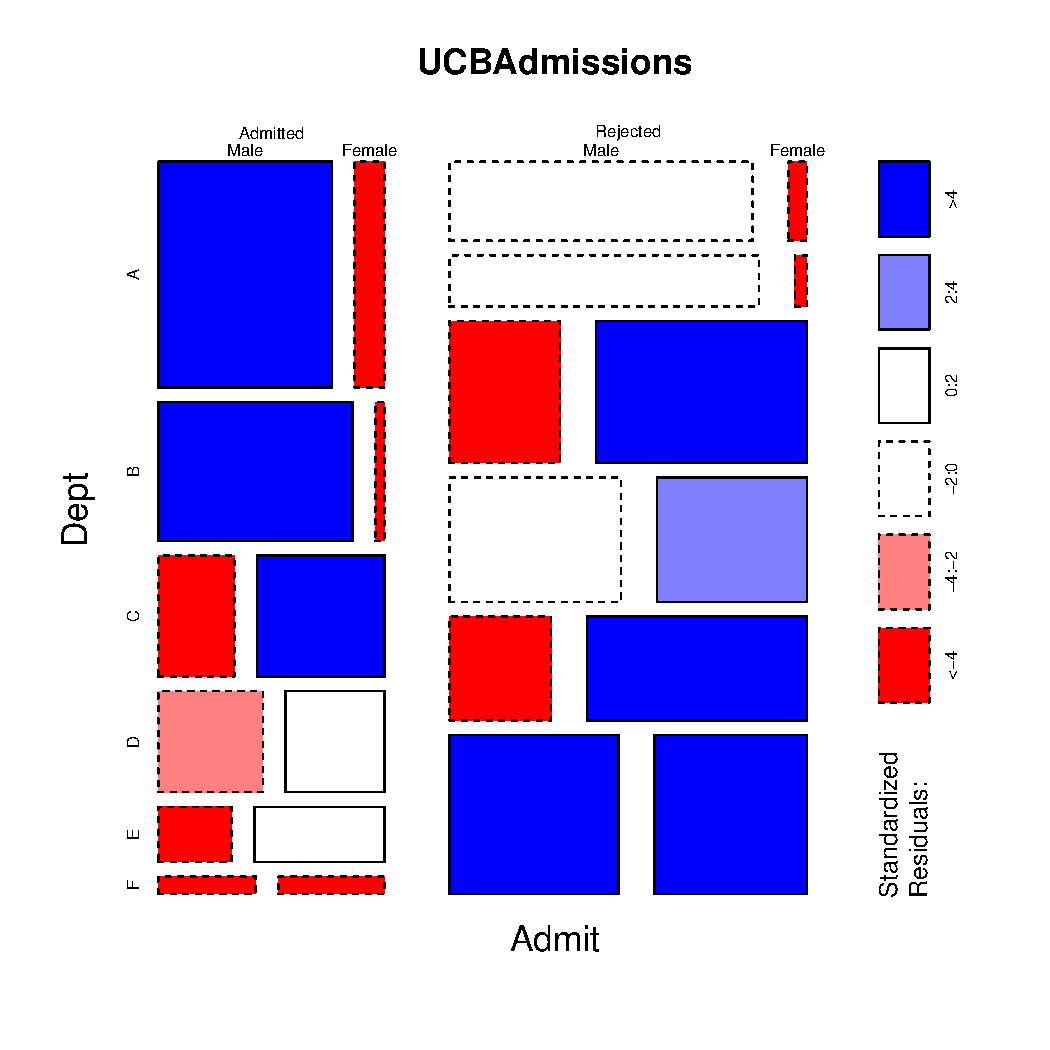
\includegraphics[width=8cm]{loglinUCBA}
\vspace*{-1em}
\caption{Mosaik-Diagramm der gemeinsamen Häufigkeiten der Kontingenztafel \lstinline!UCBAdmissions! inkl.\ Farbcodierung der Pearson-Residuen vom Modell der Unabhängigkeit.}
\label{fig:loglinUCBA}
\end{figure}

Wie in der Poisson-Regression erhält man mit \lstinline!residuals(<<loglm-Modell>>, type="<<Typ>>")! die Residuen, hier allerdings nicht pro Beobachtung, sondern pro Zelle der Kontingenztafel. Mit \lstinline!type="pearson"! sind dies die Pearson-Residuen, deren Quadratsumme gleich der Pearson-Teststatistik in der Ausgabe von \lstinline!loglm()! ist. Für zweidimensionale Kontingenztafeln ist diese Quadratsumme gleich der Teststatistik des $\chi^{2}$-Tests auf Unabhängigkeit mit \lstinline!chisq.test()! (Abschn.\ \ref{sec:chisqInd}). Analog erhält man mit \lstinline!type="deviance"! die Devianz-Residuen, deren Quadratsumme gleich der Likelihood-Ratio-Teststatistik in der Ausgabe von \lstinline!loglm()! ist.
\begin{lstlisting}
> sum(residuals(llFit, type="deviance")^2)
[1] 2097.671

> sum(residuals(llFit, type="pearson")^2)
[1] 2000.328
\end{lstlisting}

%%%%%%%%%%%%%%%%%%%%%%%%%%%%%%%%%%%%%%%%%%%%%%%%%%%%%%%%%%%%%%%%%%
%%%%%%%%%%%%%%%%%%%%%%%%%%%%%%%%%%%%%%%%%%%%%%%%%%%%%%%%%%%%%%%%%%
\subsection{Modellanpassung mit \texttt{glm()}}
\label{sec:loglinGlmFit}
%%%%%%%%%%%%%%%%%%%%%%%%%%%%%%%%%%%%%%%%%%%%%%%%%%%%%%%%%%%%%%%%%%
%%%%%%%%%%%%%%%%%%%%%%%%%%%%%%%%%%%%%%%%%%%%%%%%%%%%%%%%%%%%%%%%%%

Anders als in der Poisson-Regression liefert ein mit \lstinline!loglm()! angepasstes Modell keine Standardfehler der Parameterschätzungen. Ebenso fehlt die Möglichkeit, Konfidenzintervalle mit \lstinline!confint()! zu ermitteln. Um beides zu erhalten, lässt sich das Modell jedoch auch als Poisson-Regression mit \lstinline!glm()! formulieren. Da \lstinline!glm()! in der Voreinstellung Treatment-Kontraste verwendet, sind die Parameterschätzungen zunächst andere, mit Effektcodierung jedoch dieselben. Vorhersage und Residuen stimmen mit der des log-linearen Modells überein.
\begin{lstlisting}
# Poisson-Regression mit Treatment-Kontrasten
> glmFitT <- glm(Freq ~ Admit+Dept+Gender, family=poisson(link="log"),
+                data=UCBAdf)

> (glmTcoef <- coef(glmFitT))             # Parameterschätzungen
Coefficients:
(Intercept)  AdmitRejected     DeptB     Dept      DeptD     DeptE
    5.37111        0.45674  -0.46679  -0.01621  -0.16384  -0.46850

      DeptF  GenderFemale
   -0.26752      -0.38287

# prüfe Gleichheit der Vorhersage mit log-linearem Modell
> all.equal(c(fitted(llFit)), fitted(glmFitT), check.attributes=FALSE)
[1] TRUE
\end{lstlisting}

Auch die Teststatistik des Likelihood-Quotienten-Tests zum saturierten Modell ist im Prinzip identisch. Da \lstinline!loglm()! und \lstinline!glm()! jedoch andere numerische Optimierungsverfahren zur Maximum-Likelihood-Schätzung verwenden, sind kleine Abweichungen möglich.
\begin{lstlisting}
# saturiertes Modell mit allen Interaktionen
> glmFitT_sat <- glm(Freq ~ Admit*Dept*Gender,
+                    family=poisson(link="log"), data=UCBAdf)

> anova(glmFitT, glmFitT_sat, test="Chisq")
Analysis of Deviance Table
Model 1: Freq ~ Admit + Dept + Gender
Model 2: Freq ~ Admit * Dept * Gender
  Resid. Df Resid. Dev Df Deviance  Pr(>Chi)    
1        16     2097.7                          
2         0        0.0 16   2097.7 < 2.2e-16
\end{lstlisting}

Bei Treatment-Kontrasten ist der absolute Term gleich der Vorhersage in der Zelle, die sich als Kombination aller Referenzkategorien der beteiligten Faktoren (in der Voreinstellung jeweils die erste Faktorstufe) ergibt. Die geschätzten Koeffizienten geben jeweils die geschätzte Abweichung für eine Faktorstufe von der Referenzkategorie an.
\begin{lstlisting}
# Umrechnung mu_jk Effektcodierung aus loglm() in Treatment-Kontraste
# Zelle aus Kombination der Referenz-Kategorien
> glmTcoef["(Intercept)"]                         # Treatment-Kontraste
(Intercept)
    5.37111

> llCoef$`(Intercept)` + llCoef$Admit["Admitted"] +   # Effektcodierung
+     llCoef$Gender["Male"]  + llCoef$Dept["A"]
Admitted
 5.37111

# mu_jk für Admit = "Admit", Gender = "Female", Dept = "C"
# Treatment-Kontraste
> glmTcoef["(Intercept)"] + glmTcoef["DeptC"]+glmTcoef["GenderFemale"]
(Intercept)
   4.972034

> llCoef$`(Intercept)` + llCoef$Admit["Admitted"] +   # Effektcodierung
+     llCoef$Dept["C"] + llCoef$Gender["Female"]
Admitted
4.972034
\end{lstlisting}

Auch mit \lstinline!glm()! lassen sich die Parameter mit Effektcodierung schätzen (Abschn.\ \ref{sec:ssTypes}). Dabei fehlt die Parameterschätzung für die jeweils letzte Faktorstufe in der Ausgabe, da sie sich aus der Nebenbedingung ergibt, dass sich die Parameter pro Faktor zu Null summieren. Die Standardfehler der Parameterschätzungen sowie den zugehörigen Wald-Test extrahiert man mit \lstinline!coef(summary(<<glm-Modell>>))!. Die Einträge für den absoluten Term \lstinline!(Intercept)! sind hier ohne Bedeutung, da $\ln N$ im log-linearen Modell fest vorgegeben ist und nicht geschätzt werden muss. Konfidenzintervalle lassen sich wie gewohnt mit \lstinline!confint()! ermitteln.
\begin{lstlisting}
# Poisson-Regression mit Effektcodierung
> glmFitE <- glm(Freq ~ Admit+Dept+Gender, family=poisson(link="log"),
+                contrasts=list(Admit=contr.sum,
+                                Dept=contr.sum,
+                              Gender=contr.sum), data=UCBAdf)

# Parameterschätzungen mit Standardfehlern und Wald-Tests
> coef(summary(glmFitE))    # identisch zu loglm() Parameterschätzungen
               Estimate Std. Error    z value     Pr(>|z|)
(Intercept)  5.17756677 0.01577888 328.132716 0.000000e+00
Admit1      -0.22836970 0.01525343 -14.971696 1.124171e-50
Dept1        0.23047857 0.03071783   7.503086 6.233240e-14
Dept2       -0.23631478 0.03699431  -6.387869 1.682136e-10
Dept3        0.21427076 0.03090740   6.932668 4.129780e-12
Dept4        0.06663476 0.03272311   2.036321 4.171810e-02
Dept5       -0.23802565 0.03702165  -6.429363 1.281395e-10
Gender1      0.19143420 0.01513732  12.646505 1.169626e-36

# Konfidenzintervalle für die Relativen Raten
> exp(confint(glmFitE))     # ...
\end{lstlisting}
